\documentclass{amsart}

\usepackage{enumerate, amsmath, amsfonts, amssymb, amsthm, wasysym, graphics, graphicx, xcolor, url, hyperref, hypcap, a4wide, pdflscape, multido, xargs, colortbl, multicol, multirow, calc, shuffle}
\hypersetup{colorlinks=true, citecolor=PineGreen, linkcolor=PineGreen}
%\usepackage[all]{xy}
\usepackage{tikz}\usetikzlibrary{trees,snakes,shapes,arrows,matrix,calc}
\usepackage{comment}
\usepackage{etex}
\usepackage{ulem}\normalem % to strike through a word
\usepackage[noabbrev,capitalise]{cleveref}

%\reserveinserts{50}
\graphicspath{{figures/}}
\makeatletter
\def\input@path{{figures/}}
\makeatother

%%%%%%%%%%%%%%%%%%%%%%%%%%%%%%%%%%%%%%

\title{The lattice of acyclic pipe dreams}

\author[N.~Bergeron]{Nantel Bergeron} 
\address[N.~Bergeron]{Department of Mathematics and Statistics, York University, Toronto}
\email{bergeron@yorku.ca}
\urladdr{http://bergeron.mathstats.yorku.ca}

\author[N.~Cartier]{No\'emie Cartier} 
\address[N.~Cartier]{LRI, Université Paris Saclay}
\email{noemie.cartier@lri.fr}

\author[C.~Ceballos]{Cesar Ceballos}
\address[C.~Ceballos]{Institute of Geometry, Technische Universit\"at Graz}
\email{cesar.ceballos@tugraz.at}
\urladdr{http://www.geometrie.tugraz.at/ceballos/}

\author[V.~Pilaud]{Vincent Pilaud}
\address[V.~Pilaud]{CNRS \& LIX, \'Ecole Polytechnique, Palaiseau}
\email{vincent.pilaud@lix.polytechnique.fr}
\urladdr{http://www.lix.polytechnique.fr/~pilaud/}

%%%%%%%%%%%%%%%%%%%%%%%%%%%%%%%%%%%%%%

% theorems
\newtheorem{theorem}{Theorem}[section]
\newtheorem{corollary}[theorem]{Corollary}
\newtheorem{proposition}[theorem]{Proposition}
\newtheorem{lemma}[theorem]{Lemma}
\newtheorem{conjecture}[theorem]{Conjecture}

\theoremstyle{definition}
\newtheorem{definition}[theorem]{Definition}
\newtheorem{example}[theorem]{Example}
\newtheorem{remark}[theorem]{Remark}
\newtheorem{question}[theorem]{Question}

% newcommands
% math special letters
\newcommand{\R}{\mathbb{R}} % reals
\newcommand{\N}{\mathbb{N}} % naturals
\newcommand{\Z}{\mathbb{Z}} % integers
\newcommand{\I}{\mathbb{I}} % set of integers
\newcommand{\C}{\mathbb{C}} % set of summands

% math commands
\newcommand{\set}[2]{\left\{ #1 \;\middle|\; #2 \right\}} % set notation
\newcommand{\bigset}[2]{\big\{ #1 \;|\; #2 \big\}} % big set notation
\newcommand{\biggset}[2]{\bigg\{ #1 \;\bigg|\; #2 \bigg\}} % big set notation
\newcommand{\multiset}[2]{\left\{\!\!\left\{ #1 \;\middle|\; #2 \right\}\!\!\right\}} % multiset notation
\newcommand{\bigmultiset}[2]{\big\{\!\!\big\{ #1 \;|\; #2 \big\}\!\!\big\}} % big multiset notation
\newcommand{\ssm}{\smallsetminus} % small set minus
\newcommand{\dotprod}[2]{\langle #1 | #2 \rangle} % dot product
\newcommand{\symdif}{\triangle} % symmetric difference
\newcommand{\one}{{1\!\!1}} % the all one vector
\newcommand{\eqdef}{\mbox{\,\raisebox{0.2ex}{\scriptsize\ensuremath{\mathrm:}}\ensuremath{=}\,}} % :=
\newcommand{\defeq}{\mbox{~\ensuremath{=}\raisebox{0.2ex}{\scriptsize\ensuremath{\mathrm:}} }} % =:
\newcommand{\polar}{^\diamond} % polar
\newcommand{\simplex}{\triangle} % simplex

% operators
\DeclareMathOperator{\conv}{conv} % convex hull
\DeclareMathOperator{\cone}{cone} % cone hull
\DeclareMathOperator{\arr}{Arr} % arrangements
\DeclareMathOperator{\Inv}{Inv} % inversion set
\DeclareMathOperator{\Ninv}{Ninv} % non-inversion set
\DeclareMathOperator{\DemazureProduct}{Dem} % non-inversion set

% others
\newcommand{\fix}[1]{{\bf FIXME: }#1} % emphasis of a problem to FIX
\newcommand{\ie}{\textit{i.e.}~} % id est
\newcommand{\eg}{\textit{e.g.}~} % exempli gratia
\newcommand{\Eg}{\textit{E.g.}~} % exempli gratia
\newcommand{\aka}{\textit{aka.}~} % also known as
\newcommand{\viceversa}{\textit{vice versa}} % vice versa
\newcommand{\ordinal}{\textsuperscript{th}} % th for ordinals
\newcommand{\ex}[1]{^{\textrm{ex#1}}} % example
\newcommand{\para}[1]{\medskip\noindent\textbf{#1}} % paragraph
\newcommand{\subpara}[1]{\smallskip\noindent\textit{#1.}} % paragraph
\definecolor{PineGreen}{RGB}{2,120,120} % pinegreen color
\definecolor{darkgreen}{RGB}{57,181,74} % darkgreen color
\renewcommand{\b}[1]{{\color{blue} #1}} % blue
\renewcommand{\r}[1]{{\color{red} #1}} % red
\newcommand{\g}[1]{{\color{darkgreen} #1}} % green
\newcommand{\defn}[1]{\textbf{\textsf{\color{PineGreen} #1}}} % emphasis of a definition
\usepackage{todonotes}
\newcommand{\nantel}[1]{\todo[color=red!30]{#1 \\ \hfill --- N.}}
\newcommand{\cesar}[1]{\todo[color=orange!30,inline]{#1 \\ \hfill --- C.}}
\newcommand{\cesarm}[1]{\todo[color=orange!30]{#1 \\ \hfill --- C.}}
\newcommand{\noemie}[1]{\todo[color=green!30]{#1 \\ \hfill --- N.}}
\newcommand{\vincent}[1]{\todo[color=blue!30]{#1 \\ \hfill --- V.}}

% permutations
\newcommand{\fS}{\mathfrak{S}} % symmetric group
\newcommand{\gdproduct}{\bullet} % global descent product
\newcommand{\gdshuffle}{\shuffle_\gdproduct} % global descent shuffle product
\newcommand{\gddeconcat}{\coproduct_\gdproduct} % global descent deconcatenation coproduct
\newcommand{\HS}{{\bk\fS}} % Hopf Algebra of permutations
\newcommand{\shiftedShuffle}{\,\bar\shuffle\,} % shifted shuffle
\newcommand{\convolution}{\star} % convolution

% pipe dreams
\newcommand{\boxsize}{.35}
\newlength{\verticalOffset}
\setlength{\verticalOffset}{.3cm}
\newlength{\verticalShift}
\setlength{\verticalShift}{-.15cm}

\newcounter{length}
\newcommand{\length}[1]{%
	\setcounter{length}{0}%
	\foreach \x in {#1} {%
		\stepcounter{length}%
	}%
}

\newcommand{\pipeDreamMonoColor}[3]{% #1 = color
									% #2 = boundary color
                                    % #3 = list of types (c = cross, e = elbow, t = top, b = bottom, tb = top-bottom, or n = nothing)
	\length{#3}%
	\begin{tikzpicture}[baseline = \value{length}*\verticalShift+\verticalOffset, scale=1]
		\coordinate (origin) at (0,0);
		\newcount{\y} \y=0
		\newcount{\x}
		\foreach \line in {#3} {
			\x=0
			\foreach \t in \line {
				\coordinate (W) at ($ (origin) + ( \boxsize * \x , -\boxsize * \y ) + ( 0      , \boxsize / 2 ) $);
				\coordinate (E) at ($ (origin) + ( \boxsize * \x , -\boxsize * \y ) + ( \boxsize     , \boxsize / 2 ) $);
				\coordinate (N) at ($ (origin) + ( \boxsize * \x , -\boxsize * \y ) + ( \boxsize / 2 , \boxsize     ) $);
				\coordinate (S) at ($ (origin) + ( \boxsize * \x , -\boxsize * \y ) + ( \boxsize / 2 , 0 ) $);
				\coordinate (C) at ($ (origin) + ( \boxsize * \x , -\boxsize * \y ) + ( \boxsize / 2 , \boxsize / 2 ) $);
				\ifthenelse{\equal{\t}{e}}{
					\draw[rounded corners=\boxsize * 8, color=#1, thick] (W) -- (C) -- (N);
					\draw[rounded corners=\boxsize * 8, color=#1, thick] (S) -- (C) -- (E);			
				}{
        				\ifthenelse{\equal{\t}{c}}{
        					\draw[color=#1, thick] (W) -- (E);
        					\draw[color=#1, thick] (S) -- (N);
        				}{
        				\ifthenelse{\equal{\t}{t}}{
        					\draw[rounded corners=\boxsize * 8, color=#2] (W) -- (C) -- (N);
        					\draw[rounded corners=\boxsize * 8, color=#1, thick] (S) -- (C) -- (E);			
        				}{
        				\ifthenelse{\equal{\t}{b}}{
        					\draw[rounded corners=\boxsize * 8, color=#1, thick] (W) -- (C) -- (N);
        					\draw[rounded corners=\boxsize * 8, color=#2] (S) -- (C) -- (E);			
        				}{
        				\ifthenelse{\equal{\t}{tb}}{
        					\draw[rounded corners=\boxsize * 8, color=#2] (W) -- (C) -- (N);
        					\draw[rounded corners=\boxsize * 8, color=#2] (S) -- (C) -- (E);			
        				}{
        				\ifthenelse{\equal{\t}{n}}{}{\node at (C) {$\small \t$};}}}}}}
        				\global\advance\x by 1
			}
			\global\advance\y by 1
		}
	\end{tikzpicture}%
}

\newcommand{\pipeDreamBiColor}[4]{% #1 = colorA
                                   % #2 = colorB
                                   % #3 = boundary color
                                   % #4 = list of type/colorW/colorS (c = cross, e = elbow, or n = nothing)
	\length{#4}%
	\begin{tikzpicture}[baseline = \value{length}*\verticalShift+\verticalOffset, scale=1]
		\coordinate (origin) at (0,0);
		\newcount{\y} \y=0
		\newcount{\x}
		\foreach \line in {#4} {
			\x=0
			\foreach \t/\colorW/\colorS in \line {
				\coordinate (W) at ($ (origin) + ( \boxsize * \x , -\boxsize * \y ) + ( 0      , \boxsize / 2 ) $);
				\coordinate (E) at ($ (origin) + ( \boxsize * \x , -\boxsize * \y ) + ( \boxsize     , \boxsize / 2 ) $);
				\coordinate (N) at ($ (origin) + ( \boxsize * \x , -\boxsize * \y ) + ( \boxsize / 2 , \boxsize     ) $);
				\coordinate (S) at ($ (origin) + ( \boxsize * \x , -\boxsize * \y ) + ( \boxsize / 2 , 0 ) $);
				\coordinate (C) at ($ (origin) + ( \boxsize * \x , -\boxsize * \y ) + ( \boxsize / 2 , \boxsize / 2 ) $);
				\ifthenelse{\equal{\t}{e}}{
					\ifthenelse{\equal{\colorW}{l}}{\draw[rounded corners=\boxsize * 8, color=#1, thick] (W) -- (C) -- (N);}{}
					\ifthenelse{\equal{\colorW}{r}}{\draw[rounded corners=\boxsize * 8, color=#2, thick] (W) -- (C) -- (N);}{}
					\ifthenelse{\equal{\colorW}{b}}{\draw[rounded corners=\boxsize * 8, color=#3] (W) -- (C) -- (N);}{}
					\ifthenelse{\equal{\colorS}{l}}{\draw[rounded corners=\boxsize * 8, color=#1, thick] (S) -- (C) -- (E);}{}
					\ifthenelse{\equal{\colorS}{r}}{\draw[rounded corners=\boxsize * 8, color=#2, thick] (S) -- (C) -- (E);}{}
					\ifthenelse{\equal{\colorS}{b}}{\draw[rounded corners=\boxsize * 8, color=#3] (S) -- (C) -- (E);}{}
				}{
				\ifthenelse{\equal{\t}{c}}{
					\ifthenelse{\equal{\colorW}{l}}{\draw[color=#1, thick] (W) -- (E);}{}
					\ifthenelse{\equal{\colorW}{r}}{\draw[color=#2, thick] (W) -- (E);}{}
					\ifthenelse{\equal{\colorS}{l}}{\draw[color=#1, thick] (S) -- (N);}{}
					\ifthenelse{\equal{\colorS}{r}}{\draw[color=#2, thick] (S) -- (N);}{}
				}{
				\ifthenelse{\equal{\t}{n}}{}{\node at (C) {$\small \t$};}}}
				\global\advance\x by 1
			}
			\global\advance\y by 1
		}
	\end{tikzpicture}%
}

\newcommand{\pipeDreamTriColor}[5]{% #1 = colorA
                                   % #2 = colorB
                                   % #3 = colorC
                                   % #4 = boundary color
                                   % #5 = list of type/colorW/colorS (c = cross, e = elbow, or n = nothing)
	\length{#5}%
	\begin{tikzpicture}[baseline = \value{length}*\verticalShift+\verticalOffset, scale=1]
		\coordinate (origin) at (0,0);
		\newcount{\y} \y=0
		\newcount{\x}
		\foreach \line in {#5} {
			\x=0
			\foreach \t/\colorW/\colorS in \line {
				\coordinate (W) at ($ (origin) + ( \boxsize * \x , -\boxsize * \y ) + ( 0      , \boxsize / 2 ) $);
				\coordinate (E) at ($ (origin) + ( \boxsize * \x , -\boxsize * \y ) + ( \boxsize     , \boxsize / 2 ) $);
				\coordinate (N) at ($ (origin) + ( \boxsize * \x , -\boxsize * \y ) + ( \boxsize / 2 , \boxsize     ) $);
				\coordinate (S) at ($ (origin) + ( \boxsize * \x , -\boxsize * \y ) + ( \boxsize / 2 , 0 ) $);
				\coordinate (C) at ($ (origin) + ( \boxsize * \x , -\boxsize * \y ) + ( \boxsize / 2 , \boxsize / 2 ) $);
				\ifthenelse{\equal{\t}{e}}{
					\ifthenelse{\equal{\colorW}{l}}{\draw[rounded corners=\boxsize * 8, color=#1, thick] (W) -- (C) -- (N);}{}
					\ifthenelse{\equal{\colorW}{m}}{\draw[rounded corners=\boxsize * 8, color=#2, thick] (W) -- (C) -- (N);}{}
					\ifthenelse{\equal{\colorW}{r}}{\draw[rounded corners=\boxsize * 8, color=#3, thick] (W) -- (C) -- (N);}{}
					\ifthenelse{\equal{\colorW}{b}}{\draw[rounded corners=\boxsize * 8, color=#4] (W) -- (C) -- (N);}{}
					\ifthenelse{\equal{\colorS}{l}}{\draw[rounded corners=\boxsize * 8, color=#1, thick] (S) -- (C) -- (E);}{}
					\ifthenelse{\equal{\colorS}{m}}{\draw[rounded corners=\boxsize * 8, color=#2, thick] (S) -- (C) -- (E);}{}
					\ifthenelse{\equal{\colorS}{r}}{\draw[rounded corners=\boxsize * 8, color=#3, thick] (S) -- (C) -- (E);}{}
					\ifthenelse{\equal{\colorS}{b}}{\draw[rounded corners=\boxsize * 8, color=#4] (S) -- (C) -- (E);}{}
				}{
				\ifthenelse{\equal{\t}{c}}{
					\ifthenelse{\equal{\colorW}{l}}{\draw[color=#1, thick] (W) -- (E);}{}
					\ifthenelse{\equal{\colorW}{m}}{\draw[color=#2, thick] (W) -- (E);}{}
					\ifthenelse{\equal{\colorW}{r}}{\draw[color=#3, thick] (W) -- (E);}{}
					\ifthenelse{\equal{\colorS}{l}}{\draw[color=#1, thick] (S) -- (N);}{}
					\ifthenelse{\equal{\colorS}{m}}{\draw[color=#2, thick] (S) -- (N);}{}
					\ifthenelse{\equal{\colorS}{r}}{\draw[color=#3, thick] (S) -- (N);}{}
				}{\ifthenelse{\equal{\t}{n}}{}{\node at (C) {$\small \t$};}}}
				\global\advance\x by 1
			}
			\global\advance\y by 1
		}
	\end{tikzpicture}%
}

%\newcommand{\pipeDreamBiColor}[4]{% #1 = colorA
%                                  % #2 = colorB
%                                  % #3 = boundary color
%                                  % #4 = list of type/colorW/colorS (c = cross, e = elbow, t = top, b = bottom, tb = top-bottom, or n = nothing)
%	\length{#4}%
%	\begin{tikzpicture}[baseline = \value{length}*\verticalShift+\verticalOffset, scale=1]
%		\coordinate (origin) at (0,0);
%		\newcount{\y} \y=0
%		\newcount{\x}
%		\foreach \line in {#4} {
%			\x=0
%			\foreach \t/\colorW/\colorS in \line {
%				\coordinate (W) at ($ (origin) + ( \boxsize * \x , -\boxsize * \y ) + ( 0      , \boxsize / 2 ) $);
%				\coordinate (E) at ($ (origin) + ( \boxsize * \x , -\boxsize * \y ) + ( \boxsize     , \boxsize / 2 ) $);
%				\coordinate (N) at ($ (origin) + ( \boxsize * \x , -\boxsize * \y ) + ( \boxsize / 2 , \boxsize     ) $);
%				\coordinate (S) at ($ (origin) + ( \boxsize * \x , -\boxsize * \y ) + ( \boxsize / 2 , 0 ) $);
%				\coordinate (C) at ($ (origin) + ( \boxsize * \x , -\boxsize * \y ) + ( \boxsize / 2 , \boxsize / 2 ) $);
%				\ifthenelse{\equal{\t}{e}}{
%					\ifthenelse{\equal{\colorW}{l}}{\draw[rounded corners=\boxsize * 8, color=#1, thick] (W) -- (C) -- (N);}{\draw[rounded corners=\boxsize * 8, color=#2, thick] (W) -- (C) -- (N);}
%					\ifthenelse{\equal{\colorS}{l}}{\draw[rounded corners=\boxsize * 8, color=#1, thick] (S) -- (C) -- (E);}{\draw[rounded corners=\boxsize * 8, color=#2, thick] (S) -- (C) -- (E);}
%				}{}
%				\ifthenelse{\equal{\t}{c}}{
%					\ifthenelse{\equal{\colorW}{l}}{\draw[color=#1, thick] (W) -- (E);}{\draw[color=#2, thick] (W) -- (E);}
%					\ifthenelse{\equal{\colorS}{l}}{\draw[color=#1, thick] (S) -- (N);}{\draw[color=#2, thick] (S) -- (N);}
%				}{}
%				\ifthenelse{\equal{\t}{t}}{
%					\ifthenelse{\equal{\colorW}{l}}{\draw[rounded corners=\boxsize * 8, color=#1] (W) -- (C) -- (N);}{}
%					\ifthenelse{\equal{\colorW}{r}}{\draw[rounded corners=\boxsize * 8, color=#2] (W) -- (C) -- (N);}{}
%					\ifthenelse{\equal{\colorW}{b}}{\draw[rounded corners=\boxsize * 8, color=#3] (W) -- (C) -- (N);}{}
%					\ifthenelse{\equal{\colorS}{l}}{\draw[rounded corners=\boxsize * 8, color=#1, thick] (S) -- (C) -- (E);}{\draw[rounded corners=\boxsize * 8, color=#2, thick] (S) -- (C) -- (E);}
%				}{}
%				\ifthenelse{\equal{\t}{b}}{
%					\ifthenelse{\equal{\colorW}{l}}{\draw[rounded corners=\boxsize * 8, color=#1, thick] (W) -- (C) -- (N);}{\draw[rounded corners=\boxsize * 8, color=#2, thick] (W) -- (C) -- (N);}
%					\ifthenelse{\equal{\colorS}{l}}{\draw[rounded corners=\boxsize * 8, color=#1] (S) -- (C) -- (E);}{}
%					\ifthenelse{\equal{\colorS}{r}}{\draw[rounded corners=\boxsize * 8, color=#2] (S) -- (C) -- (E);}{}
%					\ifthenelse{\equal{\colorS}{b}}{\draw[rounded corners=\boxsize * 8, color=#3] (S) -- (C) -- (E);}{}
%				}{}
%				\ifthenelse{\equal{\t}{tb}}{
%					\ifthenelse{\equal{\colorW}{l}}{\draw[rounded corners=\boxsize * 8, color=#1] (W) -- (C) -- (N);}{}
%					\ifthenelse{\equal{\colorW}{r}}{\draw[rounded corners=\boxsize * 8, color=#2] (W) -- (C) -- (N);}{}
%					\ifthenelse{\equal{\colorW}{b}}{\draw[rounded corners=\boxsize * 8, color=#3] (W) -- (C) -- (N);}{}
%					\ifthenelse{\equal{\colorS}{l}}{\draw[rounded corners=\boxsize * 8, color=#1] (S) -- (C) -- (E);}{}
%					\ifthenelse{\equal{\colorS}{r}}{\draw[rounded corners=\boxsize * 8, color=#2] (S) -- (C) -- (E);}{}
%					\ifthenelse{\equal{\colorS}{b}}{\draw[rounded corners=\boxsize * 8, color=#3] (S) -- (C) -- (E);}{}
%				}{}
%				\global\advance\x by 1
%			}
%			\global\advance\y by1
%		}
%	\end{tikzpicture}%
%}
% cross
%\newcommand{\cross}[1][black]{\raisebox{.1cm}{\pipeDreamMonoColor{#1}{black}{c}}}
\newcommand{\cross}[1][black]{\raisebox{-.15cm}{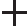
\includegraphics[scale=.9]{cross}}}
\newcommand{\crossBiColor}[2]{\raisebox{.1cm}{\pipeDreamBiColor{#1}{#2}{black}{c/l/r}}}
\newcommand{\NScross}[1][black]{\raisebox{-.15cm}{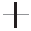
\includegraphics[scale=.9]{NScross}}}
\newcommand{\WEcross}[1][black]{\raisebox{-.15cm}{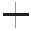
\includegraphics[scale=.9]{WEcross}}}
% elbow
%\newcommand{\elbow}[1][black]{\raisebox{.1cm}{\pipeDreamMonoColor{#1}{black}{e}}}
\newcommand{\elbow}[1][black]{\raisebox{-.15cm}{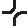
\includegraphics[scale=.9]{elbow}}}
\newcommand{\elbowBiColor}[2]{\raisebox{.1cm}{\pipeDreamBiColor{#1}{#2}{black}{e/l/r}}}
%\newcommand{\SEelbow}[1][black]{\raisebox{.1cm}{\pipeDreamBiColor{white}{#1}{black}{e/l/r}}}
\newcommand{\SEelbow}[1][black]{\raisebox{-.15cm}{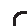
\includegraphics[scale=.9]{SEelbow}}}
%\newcommand{\WNelbow}[1][black]{\raisebox{.1cm}{\pipeDreamBiColor{#1}{white}{black}{e/l/r}}}
\newcommand{\WNelbow}[1][black]{\raisebox{-.15cm}{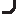
\includegraphics[scale=.9]{WNelbow}}}
\newcommand{\waving}{\mathsf{wav}}%{\raisebox{-.2cm}{\begin{tikzpicture}[scale=1]\pipeDreamBiColor{.2}{(0,0)}{black}{white}{{t/r/l},{t/l/l},{t/l/r}}\end{tikzpicture}}}
\newcommand{\transpose}{\mathsf{transp}}
\newcommand{\pipeDreams}{\Pi} % set of pipe dreams
\newcommand{\HP}{{\bk\pipeDreams}} % Hopf Algebra of pipe dreams
\newcommand{\reversingPipeDreams}{\Omega} % reversing pipe dreams
\newcommand{\contact}{^\#} % contact graph
\newcommand{\se}{\textsc{se}} % southeast
\newcommand{\nw}{\textsc{nw}} % northwest
\newcommand{\insertion}[2]{\mathsf{ins}(#1,#2)} % insertion of permutation #1 in pipe dreams with permutation #2
\newcommand{\duality}{^\star} % duality pipe dreams - triangulations
\newcommand{\acyclicPipeDreams}{\Sigma} % acyclic pipe dreams
\newcommand{\linearExtensions}{\mathcal{L}} % linear extensions
\newcommand{\noninversions}[2]{\mathsf{ninv}(#1,#2)} % non-inversions
\newcommand{\acyclicOrientations}{\Omega} % set of pipe dreams
\newcommand{\recoils}[2]{\mathsf{rec}(#1,#2)} % recoil scheme of a pipe dream
\newcommand{\canopy}[1]{\mathsf{can}(#1)} % canopy of a pipe dream
\newcommand{\greedyPipeDream}{P^{\overleftarrow{gr}}} % greedy facet
\newcommand{\antiGreedyPipeDream}{P^{\overrightarrow{gr}}} % antigreedy facet

% Subword complexes
\newcommand{\wo}{w_\circ} % longest element
\newcommand{\subwordComplex}{\mathcal{SC}} % subword complex
\newcommand{\Roots}{\mathrm{R}} % root configuration
\newcommand{\rootFunction}[2]{\mathrm{r}_{#1}(#2)} % root function
\newcommand{\subwordFacets}{\mathcal{F}} % subword complex
\newcommand{\subwordAcyclicFacets}{\mathcal{F}^{ac}} % subword complex
\newcommand{\greedyFacet}{I^{\overleftarrow{gr}}} % greedy facet
\newcommand{\antiGreedyFacet}{I^{\overrightarrow{gr}}} % antigreedy facet
\newcommand{\sweepingAlgorithm}{\mathrm{sweep}} % sweeping algorithm

% lattices
\newcommand{\meet}{\wedge} % meet
\newcommand{\join}{\vee} % join
\newcommand{\less}{\vartriangleleft} % smaller WOIP
\newcommand{\more}{\vartriangleright} % larger WOIP
\newcommand{\contactLess}[1]{\less_{#1}} % smaller contact graph
\newcommand{\contactMore}[1]{\more_{#1}} % larger contact graph
\newcommand{\projDown}{\pi_\downarrow} % Down projection
\newcommand{\projUp}{\pi^\uparrow} % Down projection


%%%%%%%%%%%%%%%%%%%%%%%%%%%%%%%%%%%%%%
%%%%%%%%%%%%%%%%%%%%%%%%%%%%%%%%%%%%%%
%%%%%%%%%%%%%%%%%%%%%%%%%%%%%%%%%%%%%%

\begin{document}

\begin{abstract}
We show that for any permutation~$\omega$, the increasing flip graph on acyclic pipe dreams with permutation~$\omega$ is a lattice quotient of the interval~$[e,\omega]$ of the weak order.
We then discuss conjectural generalizations of this result to acyclic facets of subword complexes on arbitrary finite Coxeter groups.
\end{abstract}

\maketitle

%%%%%%%%%%%%%%%%%%%%%%%%%%%%%%%%%%%%%%
%%%%%%%%%%%%%%%%%%%%%%%%%%%%%%%%%%%%%%
%%%%%%%%%%%%%%%%%%%%%%%%%%%%%%%%%%%%%%

The purpose of this note is to show that for any permutation~$\omega$, the increasing flip graph on acyclic pipe dreams with permutation~$\omega$ is a lattice quotient of the interval~$[e,\omega]$ of the weak order.
It motivates \cref{conj:Coxeter} which is the long-term perspective of this work.
The approach and proofs developed here are direct adaptations from~\cite[Sect.~1]{Pilaud-BrickAlgebra}.
\vincent{Include an introduction}
\vincent{cite \cite{BergeronBilley,KnutsonMiller-subwordComplex}}

\section{Preliminaries on pipe dreams}
\label{sec:preliminaries}

% Let $\fS_n$ denote the set of permutations of~$[n] \eqdef \{1,2,\ldots,n\}$, and let~$\fS \eqdef \bigsqcup_{n \ge 0} \fS_n$.

%%%%%%%%%%%%%%%%%%%%%%%%%%%%%%%%%%%%%%

\subsection{Pipe dreams}
\label{subsec:pipeDreams}

A \defn{pipe dream}~$P$ is a filling of a triangular shape with crosses~\cross{} and elbows~\elbow{} so that all pipes entering on the left side exit on the top side.
We only consider \defn{reduced} pipe dreams, where two pipes have at most one intersection.
We label the pipes with~$1, 2, \dots, n$ in the order of their entry points from top to bottom.
We denote by~$\omega_P \in \fS_n$ the order of the exit points of the pipes of~$P$ from left to right.
In other words, the pipe entering at row~$i$ exits at column~$\omega^{-1}_P(i)$.
For a fixed permutation~$\omega \in \fS_n$, we denote by~$\pipeDreams(\omega)$ the set of reduced pipe dreams~$P$ such that~$\omega_P = \omega$.
% We let~$\pipeDreams_n \eqdef \bigsqcup_{\omega \in \fS_n} \pipeDreams(\omega)$ and~$\pipeDreams \eqdef \bigsqcup_{n \in \N} \pipeDreams_n$.

\begin{figure}[ht]
	\centerline{
		%\documentclass[10pt]{article}
\usepackage[usenames]{color} %pour la couleur
\usepackage{amssymb} %maths
\usepackage{amsmath} %maths
\usepackage[utf8]{inputenc} %utile pour taper directement les caractères accentués
\usepackage{tikz}\usetikzlibrary{trees,snakes,shapes,arrows,matrix,calc}
\usepackage{pgfplots}
\usepackage{xifthen}
\usepackage{xcolor}
\definecolor{darkgreen}{RGB}{57,181,74} % darkgreen color

\renewcommand{\b}[1]{{\color{blue} #1}} % blue
\renewcommand{\r}[1]{{\color{red} #1}} % red
\newcommand{\g}[1]{{\color{darkgreen} #1}} % green

\newcommand{\boxsize}{.35}
\newlength{\verticalOffset}
\setlength{\verticalOffset}{.3cm}
\newlength{\verticalShift}
\setlength{\verticalShift}{-.15cm}

\newcounter{length}
\newcommand{\length}[1]{%
	\setcounter{length}{0}%
	\foreach \x in {#1} {%
		\stepcounter{length}%
	}%
}

\newcommand{\pipeDreamMonoColor}[3]{% #1 = color
									% #2 = boundary color
                                    % #3 = list of types (c = cross, e = elbow, t = top, b = bottom, tb = top-bottom, or n = nothing)
	\length{#3}%
	\begin{tikzpicture}[baseline = \value{length}*\verticalShift+\verticalOffset, scale=1]
		\coordinate (origin) at (0,0);
		\newcount{\y} \y=0
		\newcount{\x}
		\foreach \line in {#3} {
			\x=0
			\foreach \t in \line {
				\coordinate (W) at ($ (origin) + ( \boxsize * \x , -\boxsize * \y ) + ( 0      , \boxsize / 2 ) $);
				\coordinate (E) at ($ (origin) + ( \boxsize * \x , -\boxsize * \y ) + ( \boxsize     , \boxsize / 2 ) $);
				\coordinate (N) at ($ (origin) + ( \boxsize * \x , -\boxsize * \y ) + ( \boxsize / 2 , \boxsize     ) $);
				\coordinate (S) at ($ (origin) + ( \boxsize * \x , -\boxsize * \y ) + ( \boxsize / 2 , 0 ) $);
				\coordinate (C) at ($ (origin) + ( \boxsize * \x , -\boxsize * \y ) + ( \boxsize / 2 , \boxsize / 2 ) $);
				\ifthenelse{\equal{\t}{e}}{
					\draw[rounded corners=\boxsize * 8, color=#1, thick] (W) -- (C) -- (N);
					\draw[rounded corners=\boxsize * 8, color=#1, thick] (S) -- (C) -- (E);			
				}{
        				\ifthenelse{\equal{\t}{c}}{
        					\draw[color=#1, thick] (W) -- (E);
        					\draw[color=#1, thick] (S) -- (N);
        				}{
        				\ifthenelse{\equal{\t}{t}}{
        					\draw[rounded corners=\boxsize * 8, color=#2] (W) -- (C) -- (N);
        					\draw[rounded corners=\boxsize * 8, color=#1, thick] (S) -- (C) -- (E);			
        				}{
        				\ifthenelse{\equal{\t}{b}}{
        					\draw[rounded corners=\boxsize * 8, color=#1, thick] (W) -- (C) -- (N);
        					\draw[rounded corners=\boxsize * 8, color=#2] (S) -- (C) -- (E);			
        				}{
        				\ifthenelse{\equal{\t}{tb}}{
        					\draw[rounded corners=\boxsize * 8, color=#2] (W) -- (C) -- (N);
        					\draw[rounded corners=\boxsize * 8, color=#2] (S) -- (C) -- (E);			
        				}{
        				\ifthenelse{\equal{\t}{n}}{}{\node at (C) {$\small \t$};}}}}}}
        				\global\advance\x by 1
			}
			\global\advance\y by 1
		}
	\end{tikzpicture}%
}

\newcommand{\pipeDreamBiColor}[4]{% #1 = colorA
                                   % #2 = colorB
                                   % #3 = boundary color
                                   % #4 = list of type/colorW/colorS (c = cross, e = elbow, or n = nothing)
	\length{#4}%
	\begin{tikzpicture}[baseline = \value{length}*\verticalShift+\verticalOffset, scale=1]
		\coordinate (origin) at (0,0);
		\newcount{\y} \y=0
		\newcount{\x}
		\foreach \line in {#4} {
			\x=0
			\foreach \t/\colorW/\colorS in \line {
				\coordinate (W) at ($ (origin) + ( \boxsize * \x , -\boxsize * \y ) + ( 0      , \boxsize / 2 ) $);
				\coordinate (E) at ($ (origin) + ( \boxsize * \x , -\boxsize * \y ) + ( \boxsize     , \boxsize / 2 ) $);
				\coordinate (N) at ($ (origin) + ( \boxsize * \x , -\boxsize * \y ) + ( \boxsize / 2 , \boxsize     ) $);
				\coordinate (S) at ($ (origin) + ( \boxsize * \x , -\boxsize * \y ) + ( \boxsize / 2 , 0 ) $);
				\coordinate (C) at ($ (origin) + ( \boxsize * \x , -\boxsize * \y ) + ( \boxsize / 2 , \boxsize / 2 ) $);
				\ifthenelse{\equal{\t}{e}}{
					\ifthenelse{\equal{\colorW}{l}}{\draw[rounded corners=\boxsize * 8, color=#1, thick] (W) -- (C) -- (N);}{}
					\ifthenelse{\equal{\colorW}{r}}{\draw[rounded corners=\boxsize * 8, color=#2, thick] (W) -- (C) -- (N);}{}
					\ifthenelse{\equal{\colorW}{b}}{\draw[rounded corners=\boxsize * 8, color=#3] (W) -- (C) -- (N);}{}
					\ifthenelse{\equal{\colorS}{l}}{\draw[rounded corners=\boxsize * 8, color=#1, thick] (S) -- (C) -- (E);}{}
					\ifthenelse{\equal{\colorS}{r}}{\draw[rounded corners=\boxsize * 8, color=#2, thick] (S) -- (C) -- (E);}{}
					\ifthenelse{\equal{\colorS}{b}}{\draw[rounded corners=\boxsize * 8, color=#3] (S) -- (C) -- (E);}{}
				}{
				\ifthenelse{\equal{\t}{c}}{
					\ifthenelse{\equal{\colorW}{l}}{\draw[color=#1, thick] (W) -- (E);}{}
					\ifthenelse{\equal{\colorW}{r}}{\draw[color=#2, thick] (W) -- (E);}{}
					\ifthenelse{\equal{\colorS}{l}}{\draw[color=#1, thick] (S) -- (N);}{}
					\ifthenelse{\equal{\colorS}{r}}{\draw[color=#2, thick] (S) -- (N);}{}
				}{
				\ifthenelse{\equal{\t}{n}}{}{\node at (C) {$\small \t$};}}}
				\global\advance\x by 1
			}
			\global\advance\y by 1
		}
	\end{tikzpicture}%
}

\newcommand{\pipeDreamTriColor}[5]{% #1 = colorA
                                   % #2 = colorB
                                   % #3 = colorC
                                   % #4 = boundary color
                                   % #5 = list of type/colorW/colorS (c = cross, e = elbow, or n = nothing)
	\length{#5}%
	\begin{tikzpicture}[baseline = \value{length}*\verticalShift+\verticalOffset, scale=1]
		\coordinate (origin) at (0,0);
		\newcount{\y} \y=0
		\newcount{\x}
		\foreach \line in {#5} {
			\x=0
			\foreach \t/\colorW/\colorS in \line {
				\coordinate (W) at ($ (origin) + ( \boxsize * \x , -\boxsize * \y ) + ( 0      , \boxsize / 2 ) $);
				\coordinate (E) at ($ (origin) + ( \boxsize * \x , -\boxsize * \y ) + ( \boxsize     , \boxsize / 2 ) $);
				\coordinate (N) at ($ (origin) + ( \boxsize * \x , -\boxsize * \y ) + ( \boxsize / 2 , \boxsize     ) $);
				\coordinate (S) at ($ (origin) + ( \boxsize * \x , -\boxsize * \y ) + ( \boxsize / 2 , 0 ) $);
				\coordinate (C) at ($ (origin) + ( \boxsize * \x , -\boxsize * \y ) + ( \boxsize / 2 , \boxsize / 2 ) $);
				\ifthenelse{\equal{\t}{e}}{
					\ifthenelse{\equal{\colorW}{l}}{\draw[rounded corners=\boxsize * 8, color=#1, thick] (W) -- (C) -- (N);}{}
					\ifthenelse{\equal{\colorW}{m}}{\draw[rounded corners=\boxsize * 8, color=#2, thick] (W) -- (C) -- (N);}{}
					\ifthenelse{\equal{\colorW}{r}}{\draw[rounded corners=\boxsize * 8, color=#3, thick] (W) -- (C) -- (N);}{}
					\ifthenelse{\equal{\colorW}{b}}{\draw[rounded corners=\boxsize * 8, color=#4] (W) -- (C) -- (N);}{}
					\ifthenelse{\equal{\colorS}{l}}{\draw[rounded corners=\boxsize * 8, color=#1, thick] (S) -- (C) -- (E);}{}
					\ifthenelse{\equal{\colorS}{m}}{\draw[rounded corners=\boxsize * 8, color=#2, thick] (S) -- (C) -- (E);}{}
					\ifthenelse{\equal{\colorS}{r}}{\draw[rounded corners=\boxsize * 8, color=#3, thick] (S) -- (C) -- (E);}{}
					\ifthenelse{\equal{\colorS}{b}}{\draw[rounded corners=\boxsize * 8, color=#4] (S) -- (C) -- (E);}{}
				}{
				\ifthenelse{\equal{\t}{c}}{
					\ifthenelse{\equal{\colorW}{l}}{\draw[color=#1, thick] (W) -- (E);}{}
					\ifthenelse{\equal{\colorW}{m}}{\draw[color=#2, thick] (W) -- (E);}{}
					\ifthenelse{\equal{\colorW}{r}}{\draw[color=#3, thick] (W) -- (E);}{}
					\ifthenelse{\equal{\colorS}{l}}{\draw[color=#1, thick] (S) -- (N);}{}
					\ifthenelse{\equal{\colorS}{m}}{\draw[color=#2, thick] (S) -- (N);}{}
					\ifthenelse{\equal{\colorS}{r}}{\draw[color=#3, thick] (S) -- (N);}{}
				}{\ifthenelse{\equal{\t}{n}}{}{\node at (C) {$\small \t$};}}}
				\global\advance\x by 1
			}
			\global\advance\y by 1
		}
	\end{tikzpicture}%
}

\begin{document}
\pipeDreamBiColor{blue}{red}{black}{
	{n,1,3,6,5,7,2,4},
	{1,e/b/l,c/l/l,c/l/l,c/l/r,c/l/l,e/l/r,e/r/b},
	{2,e/l/l,e/l/r,c/r/l,c/r/r,c/r/l,e/r/b},
	{3,e/l/r,e/r/r,c/r/l,e/r/l,e/l/b},
	{4,e/r/r,e/r/l,e/l/l,e/l/b},
	{5,e/r/l,e/l/l,e/l/b},
	{6,e/l/l,e/l/b},
	{7,e/l/b},
}
\quad
\pipeDreamBiColor{blue}{red}{black}{
	{n,1,3,6,5,7,2,4},
	{1,e/b/l,c/l/l,c/l/l,c/l/r,c/l/l,e/l/r,e/r/b},
	{2,e/l/l,e/l/r,c/r/l,e/r/r,c/r/l,e/r/b},
	{3,e/l/r,e/r/r,c/r/l,e/r/l,e/l/b},
	{4,c/r/r,e/r/l,e/l/l,e/l/b},
	{5,e/r/l,e/l/l,e/l/b},
	{6,e/l/l,e/l/b},
	{7,e/l/b},
}
\end{document}
		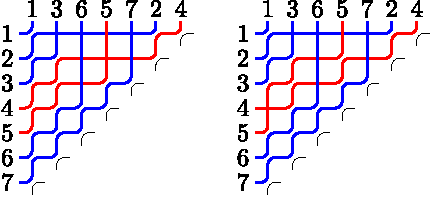
\includegraphics[scale=.9]{pipeDreams}
	}
	\caption{Two pipe dreams of~$\pipeDreams(1365724)$ connected by a flip (exchanging an elbow with the crossing on the two red pipes~$3$ and~$4$).}
	\label{fig:pipeDreams}
\end{figure}

Two pipe dreams are related by a \defn{flip} if they define the same permutation of the pipes and only differ by the position of a cross and an elbow.
An elbow~$e$ in a pipe dream~$P$ is \defn{flippable} if the two pipes passing through elbow~$e$ have a crossing~$c$, and the flip exchanges the elbow~$e$ with the cross~$c$.
See \cref{fig:pipeDreams}.
The flip is \defn{increasing} if the elbow~$e$ is weakly southwest of the crossing~$c$.
For example, the flip of \cref{fig:pipeDreams} is increasing from left to right.
%
The \defn{increasing flip graph} is the graph of increasing flips on~$\pipeDreams(\omega)$.
It is clearly a directed acyclic graph, and it has a unique source and a unique sink \cite{PilaudPocchiola}, called the \defn{greedy} and \defn{antigreedy} pipe dreams, and denoted~$\greedyPipeDream$ and~$\antiGreedyPipeDream$.
\vincent{In \cite{PilaudStump-ELlabeling}, these are called positive and negative greedy facets. Also the notations are different...}

The \defn{contact graph} of a pipe dream~$P$ is the directed graph~$P\contact$ with one node for each pipe of~$P$ and one arc for each elbow of~$P$ connecting the northwest pipe to the southeast pipe of the elbow\footnote{We have reversed the usual orientation conventions of \cite{PilaudSantos-brickPolytope, PilaudPocchiola, Pilaud-BrickAlgebra} to suit better our purposes, in particular in \cref{subsec:insertionAlgorithm}.}.
We see equivalently the contact graph~$P\contact$ as a graph on the pipes of~$P$ or on the integers~$[n]$.
We say that a pipe dream~$P$ is \defn{acyclic} if its contact graph~$P\contact$ is (no oriented cycle).
We then denote by~$\contactLess{P}$ the transitive closure of the contact graph of~$P$.
For~$\omega \in \fS_n$, we denote by~$\acyclicPipeDreams(\omega)$ the set of acyclic pipe dreams of~$\pipeDreams(\omega)$.
% We let~$\acyclicPipeDreams_n \eqdef \bigsqcup_{\omega \in \fS_n} \acyclicPipeDreams(\omega)$ and~$\acyclicPipeDreams \eqdef \bigsqcup_{n \in \N} \acyclicPipeDreams_n$.
%\vincent{Add contact graphs to \cref{fig:pipeDreams}.}


%%%%%%%%%%%%%%%%%%%%%%%%%%%%%%%%%%%%%%

\subsection{Reversing pipe dreams}
\label{subsec:reversingPipeDreams}

We say that a pipe dream~$P \in \pipeDreams_n$ is \defn{reversing} if it fixes the first pipe and reverses the order of the remaining pipes, \ie if~$\omega_P = [1, n, n-1, \dots, 2]$ (in one-line notation).
We denote by~$\reversingPipeDreams_n$ the reversing pipe dreams of~$\pipeDreams_n$.
As observed by different authors~\cite{Woo, PilaudPocchiola, Pilaud-these, Stump}, the pipe dreams of~$\reversingPipeDreams_n$ belong to the Catalan family.
\cref{fig:bijection} illustrates explicit bijections between the pipe dreams of~$\reversingPipeDreams_n$, the binary trees on $n$ vertices, and the triangulations of a convex $(n+2)$-gon.
\vincent{figure starts with pipe $0$}

\begin{figure}[h]
	\centerline{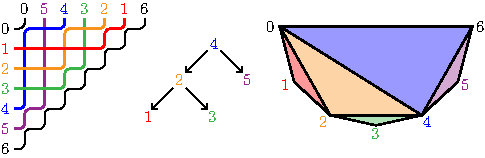
\includegraphics[scale=1.3]{dualiteTriangulation}}
	\caption{The bijection between reversing pipe dreams (left), binary trees (middle) and triangulations (right).}
	\label{fig:bijection}
\end{figure}

More precisely, the map which sends an elbow in row~$i$ and column~$j$ of the triangular shape to the diagonal~$[i,n+1-j]$ of the~$(n+2)$-gon provides the following correspondence:
\begin{center}
\begin{tabular}{r@{$\quad\longleftrightarrow\quad$}l}
pipe dream~$P \in \reversingPipeDreams_n$ & triangulation~$P\duality$ of the $(n+2)$-gon, \\
$i$th pipe of~$P$ & $i$th triangle of~$P\duality$ (with central vertex~$i$), \\
elbows of~$P$ & diagonals of~$P\duality$, \\
crosses of~$P$ & common bisectors between triangles of~$P\duality$, \\
contact graph of~$P$ & dual binary tree of~$P\duality$, \\
elbow flips in~$P$ & diagonal flips in~$P\duality$.
\end{tabular}
\end{center}

\begin{remark}
All reversing pipe dreams are acyclic.
Indeed, there contact graphs are (oriented) binary trees, which are certainly acyclic.
\end{remark}

%%%%%%%%%%%%%%%%%%%%%%%%%%%%%%%%%%%%%%

\subsection{Elementary properties of pipe dreams}
\label{subsec:elementaryProperties}

We gather in this section some elementary properties of pipe dreams needed later.
\vincent{Not sure we use all these. At least say that they are just technical points.}

\begin{lemma}
\label{lem:horiVertCrossings}
For any pipe dream~$P \in \pipeDreams(\omega)$, the pipe~$j$ of~$P$ (which enters at row~$j$ and exits at column~$\omega^{-1}(j)$) crosses
\begin{itemize}
\item vertically the pipes~$i$ such that~$i < j$ while~$\omega^{-1}(i) > \omega^{-1}(j)$,
\item horizontally the pipes~$k$ such that~$j < k$ while~$\omega^{-1}(j) > \omega^{-1}(k)$.
\end{itemize}
\end{lemma}

\begin{proof}
For~$i < j$, if~$\omega^{-1}(i) > \omega^{-1}(j)$, then the pipes~$i$ and~$j$ have to cross exactly once, while if~$\omega^{-1}(i) < \omega^{-1}(j)$ the pipes~$i$ and~$j$ cannot cross.
The same argument applies for~${k > j}$.
\end{proof}

\begin{lemma}
\label{lem:countingElbows}
For any pipe dream~$P \in \pipeDreams(\omega)$, the pipe~$j$ (which enters at row~$j$ and exits at column~$\omega^{-1}(j)$) has precisely
\begin{itemize}
\item $\noninversions{\omega}{j}$ many southeast elbows\!\SEelbow{}
\item $1+\noninversions{\omega}{j}$ many northwest elbows~\WNelbow{}
\item $j-1-\noninversions{\omega}{j}$ vertical crossings~\NScross
\item $\omega^{-1}(j)-1-\noninversions{\omega}{j}$ horizontal crossings~\WEcross
\end{itemize}
where~$\noninversions{\omega}{j} \eqdef \#\set{i \in [n]}{i < j \text{ and } \omega^{-1}(i) < \omega^{-1}(j)}$.
\end{lemma}

\begin{proof}
Pipe~$j$ enters at row~$j$ and exits at column~$\omega^{-1}(j)$, so that it passes through~$j+\omega^{-1}(j)-1$ grid points.
By \cref{lem:horiVertCrossings}, it has~$\#\set{i \in [n]}{i < j \text{ and } \omega^{-1}(i) > \omega^{-1}(j)} = j-1-\noninversions{\omega}{j}$ vertical crossings and~$\#\set{k \in [n]}{j < k \text{ and } \omega^{-1}(j) > \omega^{-1}(k)} = \omega^{-1}(j)-1-\noninversions{\omega}{j}$ horizontal crossings.
The~$1+2\,\noninversions{\omega}{j}$ remaining grid points along the pipe~$j$ are thus alternating northwest elbows and southeast elbows.
\end{proof}

\begin{lemma}
\label{lem:characterizationPipeDreams}
A collection~$P$ of~$n$ pipes pairwise disjoint except at crossing and elbows and such that for each~$j \in [n]$, the pipe~$j$ enters at row~$j$, exits at column~$\omega^{-1}(j)$, and has~$\noninversions{\omega}{j}$ southeast elbows is a pipe dream of~$\pipeDreams(\omega)$.
\end{lemma}

\begin{proof}
The argument is similar to the previous lemma.
Observe first that the pipe~$j$ must cross the paths~$i$ such that~$i < j$ and~$\omega^{-1}(i) > \omega^{-1}(j)$ and the paths~$k$ such that~$j < k$ and~$\omega^{-1}(j) > \omega^{-1}(k)$.
Moreover, it has~$\noninversions{\omega}{j}$ southeast elbows and thus~$1+\noninversions{\omega}{j}$ northwest elbows.
This already exhausts all~$j+\omega^{-1}(j)-1$ grid points of~$j$.
Therefore, the pipe~$j$ can only cross at most once any other pipe.
\end{proof}

\begin{lemma}
\label{lem:rectangle}
Let~$P$ be a pipe dream and~$i,j$ be pipes of~$P$.
If there is an elbow of pipe~$i$ weakly northwest of an elbow of pipe~$j$, then~$i \contactLess{P} j$.
\end{lemma}

\begin{proof}
Let~$x$ (resp.~$y$) be the location of an elbow of pipe~$i$ (resp.~$j$) such that~$x$ is weakly northwest of~$y$.
We proceed by induction on the grid distance from~$x$ to~$y$.
If they coincide, then pipes~$i$ and~$j$ share an elbow, so that there is an edge from~$i$ to~$j$ in~$P\contact$.
Otherwise, let~$k$ be the pipe of~$P$ with a southeast elbow at~$x$ ($k$ is either the pipe~$i$ itself, or there is an edge from~$i$ to~$k$ in~$P\contact$) and~$\ell$ be the pipe of~$P$ with a northwest elbow at~$y$ ($\ell$ is either the pipe~$j$ itself, or there is an edge from~$\ell$ to~$j$ in~$P\contact$).
Let~$R$ be the axis-parallel rectangle with elbows~$x$ and~$y$.
Since pipes~$k$ and~$\ell$ cross at most once, at least one of them has an additional elbow along the sides of~$R$.
Assume for instance that~$k$ has an elbow at~$x'$.
Then~$x'$ is still weakly northwest of~$y$ and $x',y$ are strictly closer than~$x,y$.
By induction, there is a directed path from~$k$ to~$\ell$ in~$P\contact$, and thus a path directed form~$i$ to~$j$.
\end{proof}

Note that the reciprocal assertion of \cref{lem:rectangle} is false.
We conclude by two consequences of \cref{lem:rectangle}.

\begin{lemma}
\label{lem:consequenceRectangle1}
If~$i < j$ and~$\omega^{-1}(i) < \omega^{-1}(j)$, then $i \contactLess{P} j$ for any~$P \in \pipeDreams(\omega)$.
\end{lemma}

\begin{proof}
If~$i < j$ and~$\omega^{-1}(i) < \omega^{-1}(j)$, then the pipes~$i$ and~$j$ do not cross.
Consider an elbow~$e$ of the pipe~$i$.
Since the pipe~$j$ passes southeast of~$e$, it has an elbow southeast of~$e$.
We conclude that~$i \contactLess{P} j$ by \cref{lem:rectangle}.
\end{proof}

\begin{lemma}
\label{lem:consequenceRectangle2}
Let~$P$ be a pipe dream and let~$i,j,k$ be three pipes of~$P$ such that~$\min(i,k) < j$ and~$\min(\omega^{-1}(i), \omega^{-1}(k)) < \omega^{-1}(j)$.
If~$i \to k$ in~$P\contact$, then either~$i \contactLess{P} j \contactMore{P} k$ or~$i \contactMore{P} j \contactLess{P} k$.
\vincent{not sure we really use this version}
\end{lemma}

\begin{proof}
Let~$e$ denote the contact of~$i$ and~$k$ in~$P$.
Decompose the triangular shape into three regions: the region~$A$ of all points located southwest of~$e$, the region~$B$ of all points located northwest or southeast of~$e$, and the region~$C$ of all points located northeast of~$e$.
Since~$\min(i,k) < j$ and~$\min(\omega^{-1}(i), \omega^{-1}(k)) < \omega^{-1}(j)$, the pipe~$j$ starts in region~$A$ and ends in region~$C$.
Hence, the pipe~$j$ has an elbow~$f$ in region~$B$.
We thus obtain that~$i \contactLess{P} j \contactMore{P} k$ if this $f$ is southeast of~$e$, and that~$i \contactMore{P} j \contactLess{P} k$ if $f$ is northwest of~$e$.
\end{proof}



%%%%%%%%%%%%%%%%%%%%%%%%%%%%%%%%%%%%%%
%%%%%%%%%%%%%%%%%%%%%%%%%%%%%%%%%%%%%%
%%%%%%%%%%%%%%%%%%%%%%%%%%%%%%%%%%%%%%

\section{Lattice of acyclic pipe dreams}
\label{sec:latticeAcyclicPipeDreams}

\vincent{Mention here and throughout the classical sylvester example}

The \defn{weak order} on the permutations of~$[n]$ is defined as the inclusion order of inversion sets, where an inversion of a permutation~$\pi$ is a pair of values~$i, j \in [n]$ such that~$i < j$ while~${\pi^{-1}(i) > \pi^{-1}(j)}$.
The cover relations in the weak order correspond to switching pairs of consecutive values in permutations.
The weak order is known to be a lattice \cite{GuilbaudRosenstiehl,Bjorner}.
For two permutations~$\sigma < \tau$, we denote by~$[\sigma, \tau]$ the weak order interval between~$\sigma$ and~$\tau$, which is again a lattice.

%%%%%%%%%%%%%%%%%%%%%%%%%%%%%%%%%%%%%%

\subsection{Linear extensions of pipe dreams}
\label{subsec:linearExtensions}

%Recall that a \defn{linear extension} of a binary relation~$\less$ on~$[n]$ is a permutation~$\pi \in \fS_n$ such that~$i \less j$ implies $\pi^{-1}(i) < \pi^{-1}(j)$.
%We denote by~$\linearExtensions(\less)$ the set of linear extensions of~$\less$.
%Consider an acyclic pipe dream~$P$, and recall that we denote by~$\contactLess{P}$ the transitive closure of the contact graph~$P\contact$ of~$P$.
%We denote by~$\linearExtensions(P)$ the set of linear extensions of~$\contactLess{P}$, and we say abusively that the permutations of~$\linearExtensions(P)$ are linear extensions of~$P$.
%In other words, $\pi \in \linearExtensions(P)$ if and only if~$\pi^{-1}(i) < \pi^{-1}(j)$ for all arcs~$i \to j$ in~$P\contact$.
We say that a permutation~$\pi$ is a \defn{linear extension} of a pipe dream~$P \in \pipeDreams(\omega)$ if~$\pi^{-1}(i) < \pi^{-1}(j)$ for every arc~$i \to j$ in~$P\contact$ (we should say linear extension of~$\contactLess{P}$, but prefer to simplify notation).
We denote by~$\linearExtensions(P)$ the set of linear extensions of~$P$.
%For a pipe dream~$P \in \pipeDreams(\omega)$, we denote by~$\linearExtensions(P)$ the set of \defn{linear extensions} of~$P$, \ie the permutations~$\pi$ of~$[n]$ such that~$\pi^{-1}(i) < \pi^{-1}(j)$ for every arc~$i \to j$ in~$P\contact$.
In this section, we prove the following structural property of~$\linearExtensions(P)$.

\begin{theorem}
\label{thm:partitionPipeDreams}
The set~$\set{\linearExtensions(P)}{P \in \acyclicPipeDreams(\omega)}$ partitions the weak order interval~$[e,\omega]$.
\end{theorem}

We will see in \cref{sec:algorithms} different algorithms to compute the pipe dream~$P \in \acyclicPipeDreams(\omega)$ of which a given permutation~$\pi \in [e,\omega]$ is a linear extension.
These algorithms are however not needed for the proof of \cref{thm:partitionPipeDreams}, which we break into the next three elementary lemmas.

\begin{lemma}
\label{lem:lowerSetPipeDreams}
If~$\pi \eqdef UjiV$ covers $\pi' \eqdef UijV$ in weak order, and ${\pi \in \linearExtensions(P)}$ for some~${P \in \acyclicPipeDreams(\omega)}$,~then
\begin{itemize}
\item if~$P\contact$ has no arc~$j \to i$, then~$\pi' \in \linearExtensions(P)$,
\item otherwise, $\pi' \in \linearExtensions(P')$ where~$P'$ denotes the pipe dream obtained from~$P$ by flipping the furthest northeast contact between pipes~$i$ and~$j$ in~$P$.
\end{itemize}
\end{lemma}

\begin{proof}
The first point is obvious.
For the second point, observe that the flip of the furthest contact just reverses all arcs~$j \to i$ and exchanges~$i$ and~$j$ at some extremities of the arcs of the contact graph.
\end{proof}

\begin{lemma}
\label{lem:partition}
If~$\pi \le \omega$ in weak order, then~$\pi$ a linear extension of a unique pipe dream~$P \in \acyclicPipeDreams(\omega)$.
\end{lemma}

\begin{proof}
Consider the greedy and antigreedy pipe dreams~$\greedyPipeDream$ and~$\antiGreedyPipeDream$ of \cite{PilaudPocchiola}.
For any contact between the pipes~$i$ and~$j$ in~$\greedyPipeDream$, with~$i < j$, we have
\begin{itemize}
\item if the pipes~$i$ and~$j$ never cross, then~$\omega^{-1}(i) < \omega^{-1}(j)$,
\item if the pipes~$i$ and~$j$ cross, then~$\omega^{-1}(i) > \omega^{-1}(j)$ and the contact in~$\greedyPipeDream$ must be from~$i$ to~$j$ (since all flips in~$\greedyPipeDream$ are increasing by definition).
\end{itemize}
We conclude that~$e \in \linearExtensions(\greedyPipeDream)$.
Conversely, if~$e \in \linearExtensions(P)$, all arcs of~$P\contact$ are increasing, so that all flips in~$P$ are increasing.
We conclude that~$\greedyPipeDream$ is the unique pipe dream with~$e \in \linearExtensions(\greedyPipeDream)$.
Similar arguments show that~$\antiGreedyPipeDream$ is the unique pipe dream with~$\omega \in \linearExtensions(\antiGreedyPipeDream)$.
The result thus follows from~\cref{lem:lowerSetPipeDreams}, since it shows that the existence (resp.~uniqueness) of a pipe dream~$P$ such that~$\pi \in \linearExtensions(P)$ is preserved when going down (resp.~up) in weak order.
\end{proof}

\begin{lemma}
\label{lem:interval}
If~$\pi$ is a linear extension of a pipe dream~$P \in \acyclicPipeDreams(\omega)$, then~$\pi \le \omega$ in weak order.
\end{lemma}

\begin{proof}
For any~$i < j$ with~$\omega^{-1}(i) < \omega^{-1}(j)$, the pipes~$i$ and~$j$ do not cross.
Hence, the pipe~$j$ passes southeast of every elbow of the pipe~$i$.
This shows that~$i \contactLess{P} j$ by \cref{lem:rectangle}, thus ${\pi^{-1}(i) < \pi^{-1}(j)}$.
In other words, any non-inversion of~$\omega$ is a non-inversion of~$\pi$, so that~${\pi < \omega}$.
\end{proof}

\begin{proof}[Proof of \cref{thm:partitionPipeDreams}]
Direct consequence of \cref{lem:partition,lem:interval}.
\end{proof}

%%%%%%%%%%%%%%%%%%%%%%%%%%%%%%%%%%%%%%

\subsection{Pipe dream congruence}
\label{subsec:pipeDreamCongruence}

A \defn{congruence} of a lattice~$(L, \le, \meet, \join)$ is an equivalence relation~$\equiv$ on~$L$ which respects meets and joins: $x \equiv x'$ and~$y \equiv y'$ implies $x \meet y \equiv x' \meet y'$ and~$x \join y \equiv x' \join y'$.
We will use the following classical characterization of lattice congruences.

\begin{proposition}
\label{prop:characterizationCongruences}
An equivalence relation~$\equiv$ on a lattice~$L$ is a congruence if and only if
\begin{enumerate}[(i)]
\item every equivalence class of~$\equiv$ is an interval of~$L$,
\item the projections~$\projDown : L \to L$ and~$\projUp : L \to L$, which maps an element of~$L$ to the minimal and maximal elements of its equivalence class respectively, are order preserving.
\end{enumerate}
\end{proposition}

We call \defn{pipe dream congruence} the equivalence relation~$\equiv_\omega$ on the weak order interval~$[e,\omega]$, whose equivalence classes are the sets of linear extensions of the pipe dreams of~$\acyclicPipeDreams(\omega)$.
This indeed defines an equivalence relation by \cref{thm:partitionPipeDreams}.
In this section, we prove the following statement.

\begin{theorem}
\label{thm:pipeDreamCongruence}
The pipe dream congruence~$\equiv_\omega$ is a congruence of the weak order interval~$[e,\omega]$.
\end{theorem}

We prove this statement by checking both conditions of \cref{prop:characterizationCongruences}.
For the first condition, we need the following classical characterization of weak order intervals, see \cite{BjornerWachs} or~\cite{ChatelPilaudPons}.

\begin{proposition}[{\cite[Thm.~6.8]{BjornerWachs}}]
\label{prop:WOIP}
The set~$\linearExtensions(\less)$ of linear extensions of a poset~$\less$ on~$[n]$ forms an interval~$I$ of the weak order if and only if for every~$i < j < k$,
\[
i \less k \implies i \less j \text{ or } j \less k
\qquad\text{and}\qquad
i \more k \implies i \more j \text{ or } j \more k.
\]
Moreover, the inversions of~$\min(I)$ are the pairs~$i,j \in [n]$ with $i < j$ and $i \more j$, and the non-inversions of~$\max(I)$ are the pairs~$i,j \in [n]$ with $i < j$ and $i \less j$.
\vincent{Not sure I want to use that last sentence later.}
\end{proposition}

\begin{proposition}
\label{prop:intervals}
For any pipe dream~$P \in \acyclicPipeDreams(\omega)$, the set~$\linearExtensions(P)$ is an interval of the weak order.
\end{proposition}

\begin{proof}
We just need to show that the poset~$\contactLess{P}$ (given by the transitive closure of~$P\contact$) satisfies the conditions of \cref{prop:WOIP}.
Consider~$i < j < k$ such that~$i \contactLess{P} k$.
If~$\omega^{-1}(i) < \omega^{-1}(j)$, then~$i \contactLess{P} j$ by \cref{lem:consequenceRectangle1}.
Similarly, if~$\omega^{-1}(j) < \omega^{-1}(k)$, then~$j \contactLess{P} k$ by \cref{lem:consequenceRectangle1}.
We can therefore assume that~$\omega^{-1}(i) > \omega^{-1}(j) > \omega^{-1}(k)$.
Decompose the triangular shape into three regions: the region~$A$ of all points located northeast of the last elbow of the pipe~$j$ of~$P$, the region~$B$ of all points located northwest or southeast of an elbow of the pipe~$j$ of~$P$, and the region~$C$ of all points located southwest of the first elbow of the pipe~$j$ of~$P$.
Since~$i \contactLess{P} k$, there is a path~$\pi$ form the exiting point of the pipe~$i$ of~$P$ to the entering point of the pipe~$j$ of~$P$ which travels along the pipes of~$P$, possibly jumping from the northwest pipe to the southeast pipe of an elbow it encounters.
Since~$i < j$ and~$\omega^{-1}(j) > \omega^{-1}(k)$, the path~$\pi$ starts in region~$A$ and ends in region~$C$, so that it necessarily passes from region~$A$ to region~$C$.
Since the southwest corner of~$A$ is located northeast of the northeast corner of~$C$, this forces an elbow~$e$ of~$\pi$ to lie in region~$B$.
\cref{lem:rectangle} then ensures that either~$i \contactLess{P} j$ (if~$e$ is above the pipe~$j$), or~$j \contactLess{P} k$ (if~$e$ is below the pipe~$j$).
The proof is similar if~$i \contactMore{P} k$.
\end{proof}

\begin{proposition}
\label{prop:orderPreserving}
Let $\sigma, \sigma'$ be two permutations of~$[e, \omega]$ and~$C, C'$ denote their $\equiv_\omega$-congruence classes.
Then $\sigma \le \sigma'$ implies~$\min(C) \le \min(C')$ and $\max(C) \le \max(C')$ in weak order.
\end{proposition}

\begin{proof}
We prove the statement for the maximums, the proof for the minimums is symmetrical.
Observe first that we can assume that~$\sigma$ is covered by~$\sigma'$ in weak order, so that we write~${\sigma' = \sigma s_p}$ for some simple transposition~$s_p \eqdef (p \; p+1)$.
The proof now works by induction on the weak order distance between~$\sigma$ and~$\max(C)$.
If~$\sigma = \max(C)$, the result is immediate as~${\max(C) = \sigma < \sigma' \le \max(C')}$.
Otherwise, $\sigma$ is covered by a permutation~$\tau$ in the class~$C$, and we write~$\tau = \sigma s_q$ for some simple transposition~$s_q \eqdef (q \; q+1)$.
Let~$P,P' \in \acyclicPipeDreams(\omega)$ be such that~$C = \linearExtensions(P)$ and~$C' = \linearExtensions(P')$.
We now distinguish five cases, according to the relative positions of~$p$ and~$q$:
\begin{enumerate}[(1)]
\item If~$p > q+1$, then~$\sigma = UijVk\ell W$, $\sigma' = UijV\ell kW$ and~$\tau = UjiVk\ell W$ for some~$i < j$~and~${k < \ell}$. Define~$\tau' \eqdef \sigma s_p s_q = \sigma s_q s_p = UjiV\ell kW$. By \cref{lem:lowerSetPipeDreams}, there is no arc~$i \to j$ in~$P\contact$ (since~$\sigma$ and~$\tau$ both belong to~$C$), and~$P\contact$ and~$P'{}\contact$ can only differ by arcs incident~to~$k$~or~$\ell$. Hence, there is no arc~$i \to j$ in~$P'{}\contact$. We thus obtain again by \cref{lem:lowerSetPipeDreams} that~$\tau' \in \linearExtensions(P') = C'$.
\item If~$p = q+1$, then~$\sigma = UijkV$, $\sigma' = UikjV$ and~$\tau = UjikV$ for some~$i < j < k$. Define~$\tau' \eqdef \sigma s_p s_q s_p = \sigma s_q s_p s_q = UkjiV$. Since~$\sigma \in \linearExtensions(P)$, we have~$i \not\contactMore{P} j$ and~$j \not\contactMore{P} k$, so that there is no arc~$i \to k$ in~$P\contact$ by \cref{lem:consequenceRectangle2}. By \cref{lem:lowerSetPipeDreams}, there is no arc~$i \to j$ in~$P\contact$, and~$P\contact$ and~$P'{}\contact$ can only differ by arcs incident to~$j$ or~$k$. We thus obtain that there is no arc~$i \to j$ nor~$i \to k$ in~$P'{}\contact$. Consequently, again by \cref{lem:lowerSetPipeDreams}, both~$\sigma' s_q$ and~$\tau' = \sigma' s_q s_p$ belong to~$\linearExtensions(P') = C'$.
\item If~$p = q$, then~$\sigma' = \tau$ is in~$C$, so that~$C = C'$ and there is nothing to prove.
\item If~$p = q-1$, we proceed similarly as in Situation~(2).
\item If~$p < q-1$, we proceed similarly as in Situation~(1).
\end{enumerate}
In all cases, we found~$\tau' > \tau$ with~$\tau' \in C'$.
Since~$\tau < \tau'$ with~$\tau \in C$ and~$\tau' \in C'$, and since~$\tau$ is closer to~$\max(C)$ than~$\sigma$, we obtain that ${\max(C) < \max(C')}$ by induction hypothesis.
\end{proof}

\begin{proof}[Proof of \cref{thm:pipeDreamCongruence}]
Follows from \cref{prop:characterizationCongruences}, whose conditions are guaranteed by \cref{prop:intervals,prop:orderPreserving}.
\end{proof}

%%%%%%%%%%%%%%%%%%%%%%%%%%%%%%%%%%%%%%

\subsection{Pipe dream quotient}
\label{subsec:}

For a congruence~$\equiv$ of a lattice~$L$, the \defn{lattice quotient}~$L/{\equiv}$ is the lattice on the classes of~$\equiv$ where for any two congruence classes~$X$ and~$Y$, 
\begin{itemize}
\item $X \le Y$ in~$L/{\equiv}$ if and only if there exist representatives~$x \in X$ and~$y \in Y$ such that~$x \le y$ in~$L$, or equivalently $\min(X) \le \min(Y)$, or equivalently $\max(X) \le \max(Y)$,
\item $X \meet Y$ (resp.~$X \join Y$) is the congruence classe of~$x \meet y$ (resp.~of~$x \join y$) for arbitrary representatives~$x \in X$ and~$y \in Y$.
\end{itemize}
In this section, we prove the following statement.

\begin{theorem}
\label{thm:pipeDreamQuotient}
The lattice quotient~$[e,\omega]/{\equiv_\omega}$ is isomorphic to the increasing flip poset on~$\acyclicPipeDreams(\omega)$.
\end{theorem}

To prove this result, we need the following auxiliary statement.

\begin{lemma}
\label{lem:flippable}
Consider two acyclic pipe dreams~$P,P' \in \acyclicPipeDreams(\omega)$ connected by the flip of an elbow between their pipes~$i$ and~$j$.
Then any directed path in~$P\contact$ or~$P'{}\contact$ between~$i$ and~$j$ is an arc.
\end{lemma}

\begin{proof}
Say that~$i < j$ while~$\omega^{-1}(i) > \omega^{-1}(j)$ and that~$i \to j$ is an arc of~$P\contact$ while~$j \to i$ is an arc of~$P'{}\contact$.
Since $P\contact$ is acyclic, there is no path from~$j$ to~$i$ in~$P\contact$.
Assume by means of contradiction that there is a path~$i \to k_1 \to \dots \to k_p \to j$ in~$P\contact$ with~$p \ge 1$.
Since the arcs of~$P'{}\contact$ are the arcs of~$P\contact$ where only extremities~$i$ and~$j$ can be changed, $P'{}\contact$ contains the path~$k_1 \to \dots \to k_p$ and at least one of the arcs~$i \to k_1$ or~$j \to k_1$, and at least one of the arcs~$k_p \to j$ or~$k_p \to i$.
Consequently, since~$P'{}\contact$ contains the arc~$j \to i$ and is acyclic, it must contain the path~$j \to k_1 \to \dots \to k_p \to i$.
We thus obtained that~$i \contactLess{P} k_1 \contactLess{P} j$ while~$i \contactMore{P'} k_1 \contactMore{P'} j$, and~$k_1$ has a contact with~$i$ in~$P$ and with~$j$ in~$P'$.

Consider now the elbow~$e$ of~$P$ which is a crossing in~$P'$ and the elbow~$e'$ of~$P'$ which is a crossing of~$P$.
Let~$R$ the rectangle with corners~$e$ and~$e'$.
Since~$k_1$ has a contact with~$i$ in~$P$ and with~$j$ in~$P'$, it must pass inside~$R$.
Since~$i \contactLess{P} k_1 \contactLess{P} j$ and~$i \contactMore{P'} k_1 \contactMore{P'} j$, the pipe~$k$ has no elbow located northwest or southeast of~$e$ or~$e'$, hence no elbow located north, south, west or east of~$R$.
We thus obtain that~$k$ must be straight before it reaches~$R$, and after it leaves~$R$.
Hence $k_1 < i < j$ and~$\omega^{-1}(k_1) > \omega^{-1}(j) > \omega^{-1}(i)$.
By \cref{lem:consequenceRectangle1}, this contradicts~$k_1 \contactLess{P} j$~and~$i \contactMore{P'} k_1$.
\end{proof}

\begin{proof}[Proof of \cref{thm:pipeDreamQuotient}]
It suffices to prove that the following conditions are equivalent for two distinct pipe dreams~$P,P' \in \acyclicPipeDreams(\omega)$:
\begin{enumerate}[(i)]
\item $P$ covers~$P'$ in the increasing flip poset on~$\acyclicPipeDreams(\omega)$,
\item there exist linear extensions~$\pi$ of~$P$ and~$\pi'$ of~$P'$ such that~$\pi$ covers~$\pi'$ in weak order.
\end{enumerate}
\para{(ii) $\Rightarrow$ (i)}
Follows from \cref{lem:lowerSetPipeDreams}.

\para{(i) $\Rightarrow$ (ii)}
Assume that~$P$ covers~$P'$ in the increasing flip poset.
Let~$i < j$ be the two pipes involved in the flip between~$P$ and~$P'$.
Hence, $j \to i$ is an arc of~$P$ while~$i \to j$ is an arc of~$P'$.
By \cref{lem:flippable}, there is no directed path from~$j$ to~$i$ in~$P$ besides the arcs~$j \to i$ (there might be more than one such arc).
Hence, there exists a linear extension~$\pi$ of~$P$ where~$j$ and~$i$ are consecutive.
Write~$\pi \eqdef UjiV$ and define~$\pi' \eqdef UijV$.
Since~$j \to i$ is an arc of~$P$, $\pi'$ is not a linear extension of~$P$.
Hence, by \cref{lem:lowerSetPipeDreams}, $\pi'$ is a linear extension of~$P'$.
\end{proof}

Let us conclude by providing more equivalent characterizations of the increasing flip lattice lattice on~$\acyclicPipeDreams(\omega)$.

\begin{proposition}
For any pipe dreams~$P, P' \in \acyclicPipeDreams(\omega)$, the following assertions are equivalent:
\begin{enumerate}[(i)]
\item $P < P'$ in the increasing flip poset on~$\acyclicPipeDreams(\omega)$,
\item there exist linear extensions~$\pi$ of~$P$ and~$\pi'$ of~$P'$ such that~$\pi < \pi'$ in weak order,
\item the minimal (resp.~max) linear extensions~$\pi$ of~$P$ and~$\pi'$ of~$P$ satisfy~$\pi < \pi'$ in weak order.
\item there is no~$i < j$ such that~$i \contactMore{P} j$ and~$i \contactLess{P'} j$,
\item for all~$i < j$, if~$i \contactMore{P} j$, then~$j \contactMore{P'} i$,
\item for all~$i < j$, if~$i \contactLess{P'} j$, then~$i \contactLess{P} j$,
\end{enumerate}
\end{proposition}

\begin{proof}
We already proved that (i) $\Leftrightarrow$ (ii).
\vincent{todo}
\end{proof}

%%%%%%%%%%%%%%%%%%%%%%%%%%%%%%%%%%%%%%
%%%%%%%%%%%%%%%%%%%%%%%%%%%%%%%%%%%%%%
%%%%%%%%%%%%%%%%%%%%%%%%%%%%%%%%%%%%%%

\section{Three algorithms}
\label{sec:algorithms}

\vincent{This section is in progress}
In this section, we describe three algorithms to decide whether two permutations are equivalent for the pipe dream congruence~$\equiv_\omega$.

%To sum up, there are three equivalent ways to partition the interval~$[e,\omega]$ of the weak order:
%\begin{itemize}
%\item by the sets of linear extensions~$\linearExtensions(P)$ of all pipe dreams of~$\acyclicPipeDreams(\omega)$,
%\item by the fibers of the sweeping algorithm, \vincent{choose notation}
%\item by the fibers of the insertion map~$\insertion{\cdot}{\omega}$,
%\item by the classes of the pipe dream congruence~$\equiv_\omega$.
%\end{itemize}

%%%%%%%%%%%%%%%%%%%%%%%%%%%%%%%%%%%%%%

\subsection{Sweeping algorithm}
\label{subsec:sweepingAlgorithm}

\vincent{adapt the following}
We now show that~$\linearExtensions(P) \cap \linearExtensions(P') = \varnothing$ for any two distinct acyclic pipe dreams~$P, P' \in \pipeDreams(\omega)$.
For this, we show that we can reconstructing a pipe~$P$ knowing a linear extension~$\pi \in \linearExtensions(P)$.
For this, we sweep the pipe dream in any perturbation of the northwest direction (meaning that we sweep the grid in any order such that each point is swept before all points weakly northwest of~$p$).
When we sweep a vertex~$v$ of the grid, we see a pipe~$p$ arriving horizontally at~$v$ and a pipe~$q$ arriving vertically at~$v$.
If~$p > q$, then $p$ and~$q$ already crossed before, so we have no choice but imposing an elbow at~$v$.
If~$p < q$, there are three situations:
\begin{itemize}
\item if~$\pi^{-1}(p) > \pi^{-1}(q)$ then~$p$ and~$q$ cannot touch (otherwise $\pi$ would not be a linear extension of~$P$), so that we have no choice but imposing a crossing~at~$v$,
\item if~$\omega^{-1}(p) < \omega^{-1}(q)$, then~$p$ and~$q$ cannot cross (otherwise~$P$ would not be a pipe dream of~$\pipeDreams(\omega)$), so that we have no choice but imposing a contact at~$v$,
\item if~$\pi^{-1}(p) < \pi^{-1}(q)$ and~$\omega^{-1}(p) > \omega^{-1}(q)$, then we have again two situations;
	\begin{itemize}
	\item If $q$ needs to go straight north, then we have no choice but imposing a crossing at~$v$,
	\item Otherwise, we have no choice but imposing an elbow at~$v$. Indeed, if there is a crossing at~$v$, then \cref{lem:rectangle} ensures that~$q$ will be below~$p$ in~$P\contact$, so that~$\pi$ would not be a linear extension of~$P$.
	\end{itemize}
\end{itemize}

%%%%%%%%%%%%%%%%%%%%%%%%%%%%%%%%%%%%%%

\subsection{Insertion algorithm}
\label{subsec:insertionAlgorithm}

We now define a surjective map from the permutations of~$[e, \omega]$ to the pipe dreams of~$\acyclicPipeDreams(\omega)$.
This map, adapted from~\cite{Pilaud-BrickAlgebra}, is obtained by an insertion process similar to the insertion in binary search trees.
%To properly describe this insertion algorithm, we introduce additional notations.
We now describe this insertion algorithm, which is illustrated in \cref{fig:insertionAlgorithm}.

Consider a given permutation~$\pi \eqdef \pi(1) \dots \pi(n)$ (written in one-line notation) in~$[e, \omega]$.
We start from the empty triangular shape and insert the pipes~$\pi(1), \dots, \pi(n)$ one by one in the order of the permutation~$\pi$ as northwest as possible.
In other words, at step~$t$, we consider the set~$X_t$ of free northwest elbows in the rectangle~$[\pi(t)] \times [\omega^{-1}(\pi(t))]$.
The pipe inserted at step~$t$ then starts in row~$\pi(t)$, ends in column~$\omega^{-1}(\pi(t))$, covers each elbow of~$X_t$ with a southeast elbow, and adds just one new free northwest elbow in between any two consecutive elbows of~$X_t$.
We denote the resulting pipe dream by~$\insertion{\pi}{\omega}$.
See \cref{fig:insertionAlgorithm}.

\begin{figure}[b]
	\centerline{
		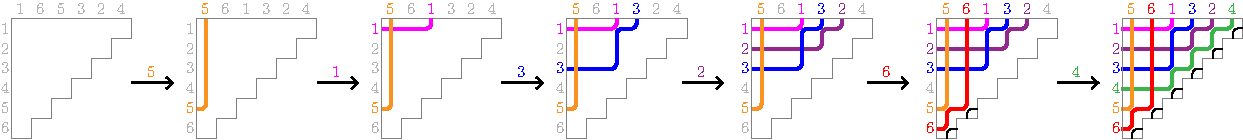
\includegraphics[scale=.9]{insertion}
	}
	\caption{The insertion~$\insertion{513264}{561324}$.}
	\label{fig:insertionAlgorithm}
\end{figure}

We need to argue that this algorithm indeed creates a pipe dream of~$\acyclicPipeDreams(\omega)$.
To see it, we observe that the following invariant is maintained throughout the algorithm.

\begin{lemma}
\label{lem:rectangleInsertionAlgorithm}
At each step~$t$ of the insertion algorithm, we have
\[
\#X_t = \# \bigset{s < t}{\pi(s) < \pi(t) \text{ and } \omega^{-1}\big( \pi(s) \big) < \omega^{-1}\big( \pi(t) \big)}.
\]
\vincent{Note that this is independent of~$\pi$... This can be seen from \cref{lem:interval}.}
\end{lemma}

\begin{proof}
Fix~$t \in [n]$.
At the beginning of the algorithm, there is no southeast elbow in the rectangle~$R_t \eqdef [\pi(t)] \times [\omega^{-1}(\pi(t))]$.
At each step~$s < t$, we have inserted a new pipe~$\pi(s)$ which enters at~$\pi(s)$ and exits at~$\omega^{-1}\big( \pi(s) \big)$.
We conclude by considering the four possible cases:
\begin{itemize}
\item If~$\pi(s) < \pi(t)$ and~$\omega^{-1}\big( \pi(s) \big) < \omega^{-1}\big( \pi(t) \big)$, then the pipe~$\pi(s)$ is completely contained in the rectangle~$R_t$. Since the pipe~$\pi(s)$ has one more northwest elbow than southeast elbow, its insertion creates a new free northwest elbow in the rectangle~$R_t$.
\item If~$\pi(s) < \pi(t)$ and~$\omega^{-1}\big( \pi(s) \big) > \omega^{-1}\big( \pi(t) \big)$, then the pipe~$\pi(s)$ enters and exits the rectangle~$R_t$ with an horizontal step, so that it has as many northwest and southeast elbows in~$R_t$, and its insertion does not modify the number of free northwest elbows in the rectangle~$R_t$.
\item If~$\pi(s) > \pi(t)$ and~$\omega^{-1}\big( \pi(s) \big) < \omega^{-1}\big( \pi(t) \big)$, then the pipe~$\pi(s)$ enters and exits the rectangle~$R_t$ with a vertical step, so that it has as many northwest and southeast elbows in~$R_t$, and its insertion does not modify the number of free northwest elbows in the rectangle~$R_t$.
\item If~$\pi(s) > \pi(t)$ and~$\omega^{-1}\big( \pi(s) \big) > \omega^{-1}\big( \pi(t) \big)$, then setting~$i = \pi(t)$ and~$j = \pi(s)$, we have~$i < j$ and~$\pi^{-1}(i) > \pi^{-1}(j)$ while~$\omega^{-1}(i) < \omega^{-1}(j)$, which contradicts our assumption that~$\pi \not< \omega$ in weak order. \qedhere
\end{itemize}
\end{proof}

\begin{corollary}
For any~$\pi \le \omega$, the insertion algorithm creates a pipe dream~$\insertion{\pi}{\omega}$ of~$\pipeDreams(\omega)$.
\end{corollary}

\begin{proof}
The algorithm constructs a collection~$P$ of $n$ pairwise disjoint pipes except at crossings and elbows.
For each~$t \in [n]$, the pipe~$\pi(t)$ enters at~$\pi(t)$, exits at~$\omega^{-1}\big( \pi(t) \big)$, and has 
\[
\# \bigset{s < t}{\pi(s) < \pi(t) \text{ and } \omega^{-1}\big( \pi(s) \big) < \omega^{-1}\big( \pi(t) \big)} = \noninversions(\omega, \pi(t))
\]
many $\se$ elbows by \cref{lem:rectangleInsertionAlgorithm} and since~$\pi < \omega$ in weak order.
We thus conclude the proof by a direct application of \cref{lem:characterizationPipeDreams}.
\vincent{Maybe we should argue that the pipes remain in the triangle.}
\end{proof}

\begin{proposition}
\label{prop:fibersInsertion}
For any pipe dream~$P \in \acyclicPipeDreams(\omega)$,  the permutations~$\pi \le \omega$ such that~$\insertion{\pi}{\omega} = P$ are precisely the linear extensions of the contact graph~$P\contact$ of~$P$.
In particular, $\insertion{\cdot}{\omega}$ is a surjection from~$[e, \omega]$ to~$\acyclicPipeDreams(\omega)$.
\end{proposition}

\begin{proof}
By construction of the insertion algorithm, all southeast elbows of the pipe~$\pi(t)$ inserted at step~$t$ are in contact with northwest elbows of pipes~$\pi(s)$ inserted at steps~$s < t$.
In other words, all edges in the contact graph of~$\insertion{\pi}{\omega}$ are of the form~$\pi(s) \to \pi(t)$ for some~$s < t$.
It follows that the permutation~$\pi$ is a linear extension of~$\insertion{\pi}{\omega}$.
Reciprocally, consider a linear extension~$\pi$ of a pipe dream~$P$.
Then~$\insertion{\pi}{\omega}$ and~$P$ have a common linear extension~$\pi$, so that~$\insertion{\pi}{\omega} = P$ by \cref{prop:partition}.
\end{proof}

In other words, the sets~$\set{\linearExtensions(P)}{P \in \acyclicPipeDreams(\omega)}$ are the fibers of the surjective insertion map~$\insertion{\cdot}{\omega}$.
Note that this concludes the proof of the surjectivity left open in \cref{prop:partition}.

%%%%%%%%%%%%%%%%%%%%%%%%%%%%%%%%%%%%%%

\subsection{Rewriting algorithm}
\label{subsec:rewritingAlgorithm}

We now characterize the sets of linear extensions of pipe dreams in terms of a rewriting rule.
We write the permutations of~$\fS_n$ as words in one-line notation.

\begin{definition}
\label{def:congruence}
For any permutation~$\omega \in \fS_n$, the \defn{pipe dream congruence} is the equivalence relation~$\equiv_\omega$ on the interval~$[e,\omega]$ of the weak order defined as the transitive closure of the rewriting rule~$U ac V \equiv_\omega U ca V$ if and only if
\[
\#\set{b \in U}{a < b < c \text{ and } \omega^{-1}(a) > \omega^{-1}(b) > \omega^{-1}(c)} \ge \#\set{b < a}{\omega^{-1}(b) < \omega^{-1}(c)},
\]
\vincent{Note that $b \in U$ on the right hand side by \cref{lem:interval}.}
where~$a, b, c$ are elements of~$[n]$ while~$U, V$ are (possibly empty) words on~$[n]$.
The letters~$b \in U$ such that~$a < b < c$ while~$\omega^{-1}(a) > \omega^{-1}(b) > \omega^{-1}(c)$ are called \defn{pipe dream congruence witnesses} for the exchange of~$a$ and~$c$.
\vincent{Another option to write this is $d \ge u$ where $d \eqdef \set{b \in U}{b > a}$ and~$u \eqdef \set{b \in U}{\omega^{-1}(b) < \omega^{-1}(c)}$.
Or $dr \ge \ell u$ where $dr \eqdef \set{b \in U}{b > a \text{ and } \omega^{-1}(b) > \omega^{-1}(c)}$ and~$\ell u \eqdef \set{b \in U}{b < a \text{ and } \omega^{-1}(b) < \omega^{-1}(c)}$.}
\end{definition}

\begin{proposition}
\label{prop:congruence}
For any~$\pi, \pi' \in [e,\omega]$, we have~${\pi \equiv_\omega \pi' \!\iff\! \insertion{\pi}{\omega} = \insertion{\pi'}{\omega} \!\iff\! \pi}$~and~$\pi'$ are linear extensions of a same pipe dream.
\end{proposition}

\begin{proof}
By \cref{prop:fibersInsertion}, each fiber of~$\insertion{\cdot}{\omega}$ gathers the linear extensions of a pipe dream of~$\pipeDreams(\omega)$.
Since the set of linear extensions of a poset is connected by simple transpositions, we just need to show that~$\pi \equiv_\omega \pi' \!\iff\! \insertion{\pi}{\omega} = \insertion{\pi'}{\omega}$ for any two permutations~$\pi = UacV$ and~$\pi' = UcaV$ of~$[e,\omega]$ which differ by the inversion of two consecutive values.

Let~$t = \pi^{-1}(a) = \pi'{-1}(c)$.
At step~$t$ of the algorithm presented in the previous section, we have inserted the word~$U$.
At that moment, let~$X_t$ (resp.~$X'_t$, resp~$Y_t$) denote the set of free northwest elbows in the rectangle~$[a] \times [\omega^{-1}(a)]$ (resp.~$[c] \times [\omega^{-1}(c)]$, resp.~$[a] \times [\omega^{-1}(c)]$).
Applying the same argument as in \cref{lem:rectangleInsertionAlgorithm}, we have
\begin{gather*}
\# Y_t = \max\big( \#\set{b \in U}{b < a \text{ and } \omega^{-1}(b) < \omega^{-1}(c)} \hspace{5cm} \\ \hspace{5cm} - \; \#\set{b \in U}{a < b < c \text{ and } \omega^{-1}(a) > \omega^{-1}(b) > \omega^{-1}(c)}, 0\big).
\end{gather*}
It follows that~$U ac V \equiv_\omega U ca V \iff \# Y_t = 0$.
However, $Y_t = 0$ if and only if all elbows of~$X_t$ are in~$[a] \times [\omega^{-1}(c), \omega^{-1}(a)]$ and all elbows of~$X'_t$ are in~$[a,c] \times [\omega^{-1}(c)]$.
The latter is equivalent to the fact that the insertion of~$a$ and~$c$ commute.
We conclude that
\[
U ac V \equiv_\omega U ca V \iff \insertion{UacV}{\omega} = \insertion{UcaV}{\omega},
\]
which concludes the proof since the set of linear extensions of a poset is connected by simple transpositions.
\end{proof}

\begin{proposition}
\label{prop:patternAvoiding}
The minimal (resp.~maximal) permutations in the partition
\(
{[e,\omega] = \bigsqcup_{P \in \acyclicPipeDreams(\omega)} \linearExtensions(P)}
\)
are the permutations avoiding the patterns~$b_1 - \cdots - b_k - ca$ (resp.~$b_1 - \cdots - b_k - ac$) where $k = \#\set{b < a}{\omega^{-1}(b) < \omega^{-1}(c)}$.
\end{proposition}

\begin{proof}
This is an immediate consequence of \cref{prop:congruence}: a permutation~$\pi$ is minimal (resp.~maximal) in its $\equiv_\omega$-congruence class if and only if it contains no consecutive exchangeable entries~$ca$ (resp.~$ac$) with~$a < c$.
\end{proof}

%%%%%%%%%%%%%%%%%%%%%%%%%%%%%%%%%%%%%%
%%%%%%%%%%%%%%%%%%%%%%%%%%%%%%%%%%%%%%
%%%%%%%%%%%%%%%%%%%%%%%%%%%%%%%%%%%%%%

\section{Canopy}
\label{sec:canopy}

Recall that the \defn{canopy} of a binary tree~$T$ with~$n$ internal nodes is the sign sequence~${\canopy{T} \in \{{-},{+}\}^{n-1}}$ defined by~$\canopy{T}_i = {-}$ if the $(i+1)$st leaf of~$T$ is a left leaf and~$\canopy{T}_i = {+}$ if the $(i+1)$st leaf of~$T$ is a right leaf.
Equivalently, $\canopy{T}_i = -$ if the node~$i$ of~$T$ is above the node~$i+1$ of~$T$ and~$\canopy{T}_i = +$ otherwise.
This map was already used by J.-L.~Loday in~\cite{LodayRonco, Loday}, but the name ``canopy'' was coined by X.~Viennot~\cite{Viennot}.
% The binary search tree insertion map and the canopy map factorize the recoil map: $\surjectionBrickZono[] \circ \surjectionPermBrick[] = \surjectionPermZono[]$. This combinatorial fact can also be understood on the geometry of the normal fans of the permutahedron, the associahedron and the cube, see \cref{subsec:normalFans}.

Before introducing the canopy, let us define the $\omega$-recoils.
For this, consider the graph~$G(\omega)$ with vertex set~$[n]$ and edge set
\[
\bigset{ij}{i < j \text{ and } j-i \le \#\set{k < i}{\omega^{-1}(k) < \omega^{-1}(j)}}.
\]
Let~$\acyclicOrientations(\omega)$ denote the set of acyclic orientations of~$G(\omega)$.

\begin{definition}
The \defn{$\omega$-recoil scheme} of a permutation~$\pi \in [e,\omega]$ is the orientation~${\recoils{\pi}{\omega} \in \acyclicOrientations(\omega)}$ where for all~$i < j \in [n]$ such that~$j-i \le \#\set{k < i}{\omega^{-1}(k) < \omega^{-1}(j)}$, the edge~$ij$ is oriented~$i \to j$ if~$\pi^{-1}(i) < \pi^{-1}(j)$ and~$j \to i$ if~$\pi^{-1}(j) < \pi^{-1}(i)$.
We call \defn{$\omega$-recoil map} the map~$\recoils{\cdot}{\omega} : [e,\omega] \to \acyclicOrientations(\omega)$.
\end{definition}

\begin{remark}
The fiber of an acyclic orientation~$O \in \acyclicOrientations(\omega)$ under the $\omega$-recoil map~$\recoils{\cdot}{\omega}$ are the linear extensions of~$O$ in~$[e,\omega]$.
\end{remark}

We now define a generalization of the canopy map for pipe dreams in~$\acyclicPipeDreams(\omega)$.
To ensure that \cref{def:canopy} is valid, we need the following simple observation on comparisons of ``close'' pipes in a pipe dream.

\begin{lemma}
\label{lem:canopy}
If~$i < j$ satisfy~$j-i \le \#\set{k < i}{\omega^{-1}(k) < \omega^{-1}(j)}$, then the pipes~$i$ and~$j$ in any acyclic pipe dream~$P \in \acyclicPipeDreams(\omega)$ are comparable~for~$\contactLess{P}$.
\end{lemma}

\begin{proof}
If pipes~$i$ and~$j$ were incomparable in~$\contactLess{P}$, there would be two $\equiv_\omega$-congruent permutations~$UijV \equiv_\omega UjiV$.
However, the assumption contradicts the definition of the $\equiv_\omega$-conguence in \cref{def:congruence}.
\end{proof}

\begin{definition}
\label{def:canopy}
The \defn{canopy} of a pipe dream~$P \in \acyclicPipeDreams(\omega)$ is the orientation~$\canopy{P} \in \acyclicOrientations(\omega)$ where for all~$i < j \in [n]$ such that~$j-i \le \#\set{k < i}{\omega^{-1}(k) < \omega^{-1}(j)}$, the edge~$ij$ is oriented~$i \to j$ if~$i \contactLess{P} j$ and~$j \to i$ if~$j \contactLess{P} i$.
It indeed defines an acyclic orientation of~$G(\omega)$ by \cref{lem:canopy}.
We call \defn{canopy} the map~$\canopy{\cdot}: \acyclicPipeDreams(\omega) \to \acyclicOrientations(\omega)$.
\end{definition}

\begin{proposition}
\label{prop:latticeHomomorphisms}
The maps~$\recoils{\cdot}{\omega}$, $\insertion{\cdot}{\omega}$, and~$\canopy{\cdot}$ define the following commutative diagram of lattice homomorphisms:
\[
\begin{tikzpicture}
  \matrix (m) [matrix of math nodes,row sep=1.2em,column sep=5em,minimum width=2em]
  {
     [e,\omega]  	&								& \acyclicOrientations(\omega)	\\
					& \acyclicPipeDreams(\omega) 	&								\\
  };
  \path[->] (m-1-1) edge node [above] {$\recoils{\cdot}{\omega}$} (m-1-3);
  \path[->>] (m-1-1) edge node [below] {$\insertion{\cdot}{\omega}\qquad$} (m-2-2.west);
  \path[->] (m-2-2.east) edge node [below] {$\quad\canopy{\cdot}$} (m-1-3);
\end{tikzpicture}
\]
\end{proposition}

\begin{proof}
Consider a permutation~$\pi$ and let~$i < j \in [n]$ be such that~$j-i \le \#\set{k < i}{\omega^{-1}(k) < \omega^{-1}(j)}$.
Assume that the edge~$ij$ is oriented from~$i$ to~$j$.
Then~$\pi^{-1}(i) < \pi^{-1}(j)$, thus the pipe~$i$ is inserted before the pipe~$j$ in~$\insertion{\pi}{\omega}$, so that~$i \contactLess{\insertion{\pi}{\omega}} j$ and there is also an arc from~$i$ to~$j$ in~$\canopy{\insertion{\pi}{\omega}}$.
\end{proof}

%%%%%%%%%%%%%%%%%%%%%%%%%%%%%%%%%%%%%%
%%%%%%%%%%%%%%%%%%%%%%%%%%%%%%%%%%%%%%
%%%%%%%%%%%%%%%%%%%%%%%%%%%%%%%%%%%%%%

\section{Future work}
\label{sec:futureWork}

%%%%%%%%%%%%%%%%%%%%%%%%%%%%%%%%%%%%%%

\subsection{Sortability and alignement}

We should describe the minimum (or maximum) of the congruence classes of~$\equiv_\omega$ by
\begin{itemize}
\item a pattern avoiding condition, see \cref{prop:patternAvoiding}.
\item ``$\omega$-sortability'', see~\cite{Reading-sortableElements}.
\item ``$\omega$-alignement'', see~\cite{Reading-sortableElements}.
\end{itemize}

\subsection{Other Coxeter groups}

\vincent{This part is not up-to-date.  We have new (hopefully correct) conjectures.}
All the arguments presented above should extend to type A Cambrian pipe dreams... This means that we consider the increasing flip poset of the type~$A$ subword complex~$\subwordComplex(\wo(c),\omega)$ for any Coxeter element~$c$ and any permutation~$\omega$ of~$\fS_n$. Similar arguments where already developed in~\cite{Pilaud-BrickAlgebra} for the particular case of the permutation
\[
\omega = [1, \dots, k, n-k, n-k-1, \dots, k+2, k+1, n-k+1, \dots, n].
\]
More generally, we can consider the following conjecture.

\begin{conjecture}
\label{conj:Coxeter}
For any finite Coxeter group~$W$, any Coxeter element~$c$ of~$W$, and any element~$w \in W$, the increasing flip poset on the acyclic facets of the subword complex~$\subwordComplex(\wo(c),w)$ is a lattice quotient of the interval~$[e,w]$ of the weak order on~$W$.
\end{conjecture}

Let's be a little more precise here: for an acyclic facet~$F$ of the subword complex~$\subwordComplex(\wo(c),w)$, one can consider the set~$\set{\pi \in W}{\R_{\ge 0} \pi(\Delta) \supseteq \R_{\ge 0} \Roots(F)}$, \ie the elements of~$W$ whose dual Coxeter chamber belongs to the cone generated by the root configuration of~$F$. I hope that this defines a lattice congruence of~$[e,w]$.

We should actually consider the lattice properties of the acyclic facets of~$\subwordComplex(c^k\wo(c),w)$ for any~$k$ and any~$w$. In type~$A$, this is the same as any subword complex~$\subwordComplex(c^k\wo(c),w)$ can be embedded in a bigger~$\subwordComplex(\wo(c'),w')$. In other types however it is a more general question.

%%%%%%%%%%%%%%%%%%%%%%%%%%%%%%%%%%%%%%

\subsection{Hopf algebra}

Define an equivalence relation~$\equiv$ on intervals~$[\pi,\omega]$ of the weak order by~$[\pi,\omega] \equiv [\pi',\omega'] \iff \omega = \omega' \text{ and } \pi \equiv_\omega \pi'$. Essentially, we proved that the collection of all acyclic pipe dreams is in bijection with the equivalence classes of~$\equiv$. Now is there a Hopf algebra on intervals of the weak order such that the equivalence relation~$\equiv$ gives a subalgebra?
\vincent{I believe that this part should disappear.}

%%%%%%%%%%%%%%%%%%%%%%%%%%%%%%%%%%%%%%

\subsection{Subword complexes}
\label{subsec:subwordComplexes}

Pipe dreams are a very particular family of the family of subword complexes.
Consider a Coxeter system~$(W,S)$, where~$W$ is a finite Coxeter group and~$S$ is the set of simple reflections of~$W$.
We denote by~$e$ (resp.~$\wo$) the identity (resp.~longest element) of~$W$.
Let~$Q \eqdef q_1 \dots q_m \in S^*$ be a word on the alphabet formed by the simple generators of~$W$ and~$w \in W$.
The \defn{subword complex}~$\subwordComplex(Q,w)$ is the simplicial complex whose ground set~$[m]$ are the positions in~$Q$ and whose facets are the complements of the reduced expressions for~$w$ in~$Q$.

It is known that~$\subwordComplex(Q,w)$ is either a ball or a sphere, in particular it is a pseudomanifold (with or without boundary).
The flip graph of~$\subwordComplex(Q,w)$ is the graph whose vertices are the facets of~$\subwordComplex(Q,w)$ and whose edges are the ridges of~$\subwordComplex(Q,w)$.
If~$F,F'$ are two adjacent facets with~$F \ssm \{p\} = F' \ssm \{p'\}$, we say that the flip is \defn{increasing} when~$p < p'$.
The increasing flip graph was studied in particular in~\cite{PilaudStump-ELlabelings}.
It is known to be acyclic, and its transitive closure is an EL-shellable poset (see~\cite{PilaudStump-ELlabelings} for the precise definition and references).

There is also a notion of acyclicity for subword complexes.
It is based on the notion of \defn{root configuration}~$\Roots(F)$ of a facet~$F$ of~$\subwordComplex(Q,w)$.
We skip the details and refer to~\cite{CeballosLabbeStump, PilaudStump-brickPolytope} for details.
The facet~$F$ is \defn{acyclic} if its root configuration is pointed (meaning that it generates a pointed cone).

\begin{example}
Consider the symmetric group~$\fS_{n+1}$ generated by the set of simple transpositions $\set{\tau_i}{i \in [n]}$ where~$\tau_i \eqdef (i \; i+1)$.
For a permutation~$\omega \in \fS_{n+1}$, the pipe dreams of~$\pipeDreams(\omega)$ correspond to the facets of the subword complex~$\subwordComplex(Q,\omega)$ with~$Q = \tau_1, \tau_2, \dots, \tau_n, \tau_1, \tau_2, \dots, \tau_{n-1}, \dots, \tau_1, \tau_2, \tau_1$.
% The notions of flips, increasing flips and acyclic pipe dreams transpose in the world of subword complexes.
\end{example}

\begin{example}
For any Coxeter group~$W$ and any Coxeter element~$c \in W$ (a product of all generators of~$S$ in a given arbitrary order), let~$\wo(c)$ denote the $c$-sorting word of~$\wo$ (see \cite{Reading-CambrianLattices} for details).
Extending the observation of \cref{subsec:reversingPipeDreams}, it was shown in~\cite{CeballosLabbeStump} that the subword complex~$\subwordComplex(c\wo(c), \wo)$ is isomorphic to the cluster complex of type~$W$.
In particular, the increasing flip graph is the Hasse diagram of the $c$-Cambrian lattice of~\cite{Reading-CambrianLattices}.
\end{example}

In contrast to the previous example, consider the word~$Q = \tau_1 \tau_2 \tau_3 \tau_2 \tau_1 \tau_2 \tau_3 \tau_2 \tau_1$ on the simple generators of the symmetric group~$\fS_4$ and the subword complex~$\subwordComplex(Q,\wo)$.
Note that all facets in this subword complex are acyclic.
It is shown in~\cite[Rem.~5.12]{PilaudStump-brickPolytope} that its increasing flip poset is not a lattice.
This shows that neither the increasing flip poset, nor the acyclic increasing flip poset are lattices in general, even in type~$A$.
In this note, we investigate the case of acyclic pipe~dreams.

%%%%%%%%%%%%%%%%%%%%%%%%%%%%%%%%%%%%%%
%%%%%%%%%%%%%%%%%%%%%%%%%%%%%%%%%%%%%%
%%%%%%%%%%%%%%%%%%%%%%%%%%%%%%%%%%%%%%

\newpage
\section{Subword complexes}

The objective of this section is to partially extend the results about the lattice structure of acyclic pipe dreams, presented in \cref{sec:latticeAcyclicPipeDreams}, to the wider context of subword complexes of finite type.
Before doing so, we recall some preliminaries about finite Coxeter groups and subword complexes.
We refer to~\cite{BjornerBrenti, Humphreys} for more details on Coxeter groups. 

%%%%%%%%%%%%%%%%%%%%%%%%%%%%%%%%%%%%%%

\subsection{Finite coxeter groups} 
%a~\cesar{To do:\\
%Coxeter groups of finite type, root systems, weak order, Bruhat order, inversions, non-inversions. 
%}
We consider a \defn{finite root system} $\Phi=\Phi^+\cup \Phi^-$ in an $n$-dimensional euclidian space $V$, with \defn{simple roots} $\Delta=\{\alpha_1,\dots,\alpha_n\} \subseteq \Phi^+$.
The reflections along the hyperplanes orthogonal to the roots in $\Phi$ generate a finite Coxeter group $W$. 
This group is generated by the simple transpositions $S=\{s_1,\dots ,s_n\}$, where $s_i$ is the reflection along the hyperplane orthogonal to the simple root $\alpha_i$.
We also denote by $\alpha_s$ the simple root associated to $s\in S$.
Throughout this paper, we only consider Coxeter groups which are finite.
They are classified in terms of Dynkin diagrams, and arise from finite root systems, see~\cite{Humphreys}. 

Abstractly, the \defn{Coxeter group} $W$ is the group generated by a collection $S=\{s_1,\dots, s_n\}$ which satisfies the relations $(s_is_j)^{m_{ij}}=1$, where $m_{ii}=1$ and $m_{ij}\geq 2$ for~$i\neq j$.
The pair $(W,S)$ is called a \defn{Coxeter system}.
The \defn{length} $\ell(w)$ of an element $w\in W$ is the smallest~$\ell$ such that it can be written of the form $w=w_1w_2\dots w_\ell$ where $w_i\in S$.
A \defn{reduced expression} of~$w$ is an expression of minimal length.
We denote by $\wo$ the \defn{unique longest} element in $W$.

For a finite Coxeter $W$ associated to a root system $\Phi$, the length $\ell(w)$ can be geometrically interpreted as the cardinality of the \defn{inversion set} $\Inv(w)$ of $w$, which is defined as
\begin{align}\label{def_inversionset}
\Inv(w) \eqdef \Phi^+ \cap w(\Phi^-).
\end{align}
Indeed, this set can be written as 
\begin{align}\label{def_inversionset2}
\Inv(w) \eqdef \{\alpha_{w_1}, w_1(\alpha_{w_2}),\dots , w_1w_2\dots w_{\ell-1}(\alpha_{w_\ell})\}
\end{align}
for any reduced expression $w=w_1w_2\dots w_\ell$ of $w$.

The \defn{non-inversion set} $\Ninv (w)$ of $w$ is defined as
\begin{align}
\Ninv(w) & \eqdef \Phi^+ \cap w(\Phi^+) \label{def_noninversionset} \\
& =\Inv(w\wo)
\end{align}

In particular, 
\begin{align}
\Phi^+=\Inv(w) \sqcup \Ninv (w).
\end{align}

The \defn{weak order} on $W$ is the partial order $\leq$ defined by $u \leq w$ if there exists $v \in W$ such that $uv = w$ and $\ell(u) + \ell(v) = \ell(w)$.
In other words, the element $w$ has a reduced expression with a prefix which is a reduced expression of $u$.
Equivalently, the weak order corresponds to the inclusion order on inversion sets, that is $u \leq w$ if and only if $\Inv(u) \subseteq \Inv(w)$.
This order defines a lattice structure on the elements of W.
The minimal element is the identity $e \in W$ and the maximal element is $\wo$.


\subsection{Subword complexes}
%~\cesar{To do:\\
%subword complexes, flips, greedy facets, \sout{root function, root configuration, acyclic facets}. 
%}

Motivated by their study of Gröbner geometry of Schubert varieties~\cite{KnutsonMiller-GroebnerGeometry}, Knutson and Miller~\cite{KnutsonMiller-subwordComplex} introduced a remarkable family of simplicial complexes in the context of Coxeter groups.

Let $(W,S)$ be a Coxeter system of finite type, $Q=(q_1,\dots,q_m)$ be a word in the generators $S$, and $w\in W$ be an element of the group.
For $J\subseteq [r]$, we denote by $Q_J$ the subword of~$Q$ consisting of the letters with positions in $J$.
The \defn{subword complex} $\subwordComplex(Q,w)$ is the simplicial complex whose facets are subsets $I\subseteq [m]$ such that $Q_{[m]\setminus I}$ is a reduced expression for $w$.
We denote the \defn{set of facets} of $\subwordComplex(Q,w)$ by $\subwordFacets(Q,w)$.

Two facets $I,J\in\subwordComplex(Q,w)$ are said to be connected by a \defn{flip} if they differ one element:
\[J=I\smallsetminus \{i\} \cup\{j\}\]
for some $i\in I$ and $j\in J$ with $i\neq j$.
If $i<j$, the flip from $I$ to $J$ is called an \defn{increasing flip}.

The increasing flip graph on facets of the subword complex is an acyclic graph which has a unique source and a unique sink~\cite{Pilaud-greedyFlipTree, PilaudStump-ELlabelings}.
These two special facets are called the \defn{greedy facet} $\greedyFacet$ and the \defn{antigreedy facet} $\antiGreedyFacet$.
They are the lexicographically smallest and largest facets of $\subwordComplex(Q,\pi)$, respectively.

The poset on the set of facets induced by increasing flips is called the \defn{increasing flip poset}.

\begin{definition}[{\cite{CeballosLabbeStump}}]
    The \defn{root function} $\rootFunction{I}{\cdot}:[m]\rightarrow \Phi$ associated to a facet $I$ is the map from positions in the word $Q$ to roots defined by 
    \[
    \rootFunction{I}{k} \eqdef \prod Q_{[k-1]\smallsetminus I}(\alpha_{q_k}).
    \]
    The \defn{root configuration} is the set $\Roots(I)=\set{\rootFunction{I}{i}}{i\in I}$.
    The facet $I$ is called \defn{acyclic} if $\cone \Roots(I)$ is a pointed cone.
    We denote the \defn{set of acyclic facets} by $\subwordAcyclicFacets(Q,w)$.
\end{definition}

The root function is a useful and well established tool in the study of subword complexes.
For instance, they can be used to fully understand flips.

\begin{lemma}[{\cite{CeballosLabbeStump, KnutsonMiller-subwordComplex}}]
\label{lem_rootfunction_flips}
Let $I$ be a facet of the subword complex~$\subwordComplex(Q,w)$.
The following hold:
\begin{enumerate}
    \item $i \in I$ is flippable if and only if $\pm \rootFunction{I}{i} \in \Inv(w)$.
    \item If $i \in I$ is flippable, it can be flipped to the unique $j\in [m]\smallsetminus I$ such that $\rootFunction{I}{j} = \pm\rootFunction{I}{i}$.
    The flip is increasing ($i<j$) when $\rootFunction{I}{i}\in \Phi^+$ and decreasing ($i>j$) when $\rootFunction{I}{i}\in \Phi^-$.\label{lem_rootfunction_flips2}
    \item If $I'=I\smallsetminus \{i\}\cap \{i'\}$ is a facet obtained from $I$ by flipping $i$ to $i'$ with $i<i'$, then
    \begin{equation}\label{eq_rootfunction_flip}
         \rootFunction{I'}{k} = 
  \begin{cases}
    s_\beta(\rootFunction{I}{k}), & \text{for } i < k \leq i' \\
    \rootFunction{I}{k}, & \text{otherwise}
  \end{cases}
    \end{equation}
    where $\beta=\rootFunction{I}{i}$ and $s_\beta\in W$ is the reflection orthogonal to the root $\beta$.
    \item $i \in I$ is not flippable if and only if $\rootFunction{I}{i}\in \Ninv(w)$.
\end{enumerate}
\end{lemma}

\subsection{Linear extensions of facets}

\begin{definition}
Let $\subwordComplex(Q,w)$ be a non-empty subword complex and $I\in \subwordComplex(Q,w)$ be a facet.
An element $\pi\in W$ is called a \defn{linear extension} of $I$ if the root configuration $\Roots(I)\subseteq \pi(\Phi^+)$.
The \defn{set of linear extensions} of $I$ is denoted by
\begin{align}
\linearExtensions(I)=
\set{\pi\in W}{\Roots(I)\subseteq \pi(\Phi^+)}.   
\end{align}
\end{definition}

\begin{lemma}
\label{lem_acyclic_nonempty}
$\linearExtensions(I)\neq \varnothing$ if and only if $I$ is acyclic.
\end{lemma}
\begin{proof}
Let $\Phi=\Phi^+\sqcup\Phi^-$ be the root system associated to $W$.
A known result for root systems of finite type states that any other choice of a positive root system $\Phi^+$ for $\Phi$ is of the form $\widetilde \Phi^+=\pi(\Phi^+)$ for some $w\in W$.
Since any pointed cone is contained in some $\widetilde \Phi^+$, then 
\[
\begin{array}{rcl}
I \text{ is acyclic}  & \longleftrightarrow  &  \cone \Roots(I) \text{ is pointed} \\
  & \longleftrightarrow  & \cone \Roots(I)\subseteq \pi(\Phi^+) \text{ for some } \pi\in W \\
  & \longleftrightarrow  &  \Roots(I)\subseteq \pi(\Phi^+) \text{ for some } \pi\in W \\
  & \longleftrightarrow  &  \linearExtensions(I) \neq \varnothing 
\end{array}
\]
\end{proof}

\begin{lemma}
\label{lem_pi_phiplus_inv_ninv}
The following holds,
\[
\pi(\Phi^+)=-\Inv(\pi)\sqcup \Ninv(\pi).
\]
\end{lemma}

\begin{proof}
This is straight forward from the definition of inversions and non-inversion of $\pi$.
In fact, multiplying Equation~\eqref{def_inversionset} by $-1$ we deduce $\pi(\Phi^+)\cap \Phi^-=-\Inv(\pi)$.
Furthermore,  
$\pi(\Phi^+)\cap \Phi^+=\Ninv(\pi)$ by Equation~\eqref{def_noninversionset}.
\end{proof}

The following lemma regards linear extensions of the greedy and antigreedy facets.

\begin{lemma}\label{lem_linearext_greedyfacets}
    Let $\greedyFacet$ and $\antiGreedyFacet$ be the greedy and antigreedy facets of $\subwordComplex(Q,w)$, respectively.
Then 
    \begin{enumerate}
        \item $e\in \linearExtensions(\greedyFacet)$.
        \item $w \in \linearExtensions(\antiGreedyFacet)$.
        \item If $e\in \linearExtensions(I)$ then $I=\greedyFacet$.
    \end{enumerate}
\end{lemma}
\begin{proof}
    Let $e\in W$ be the minimal element of the week order.
    The greedy facet $\greedyFacet$ is the unique facet for which every flip (if any) is increasing.
By \cref{lem_rootfunction_flips}~\eqref{lem_rootfunction_flips2}, this implies that $\greedyFacet$ is the unique facet $I$ such that $\Roots(I)\subseteq \Phi^+ = e(\Phi^+)$.
This proves parts (1) and (3) of the Lemma.   
    
    For part (2) we need to analyze the possibilities for the set $\Roots(\antiGreedyFacet)$.
 By \cref{lem_rootfunction_flips}~\eqref{lem_rootfunction_flips2}, if $i\in \antiGreedyFacet$ is flippable then $\rootFunction{\antiGreedyFacet}{i}\in -\Inv(w)$.
Furthermore, if $i\in \antiGreedyFacet$ is not flippable then $\rootFunction{\antiGreedyFacet}{i}\in \Ninv(w)$.
Therefore, $\Roots(\antiGreedyFacet)\subseteq w(\Phi^+)=-\Inv(w)\sqcup \Ninv(w)$.
\end{proof}

\begin{remark}
The concept of linear extensions of acyclic facets of subword complexes are a natural generalization of linear extensions of contact graphs of acyclic pipe dreams that we introduced in \cref{subsec:linearExtensions}.
Indeed ... 
\cesar{make this connection crystal clear...}
\end{remark}


\subsection{Two fundamental theorems about linear extensions}
In this section, we present our two main results about linear extensions for subword complexes, \cref{thm_subword_linearextensions_A} and \cref{thm_subword_linearextensions_B}.

We say that a subset $A$ of the weak order is a \defn{lower set} if $a<b$ and $b\in A$ implies $a\in A$.
We say that $A$ is \defn{closed by intervals} if $a,b\in A$ implies that $[a,b]\in A$, where $[a,b]=\{c: a \leq c\leq b\}$.
\vincent{I usually say ``order-convex''}

\begin{theorem}\label{thm_subword_linearextensions_A}
Let~$\subwordComplex(Q,w)$ be a non-empty subword complex.
The following hold:
\begin{enumerate}
\item  $\bigcup_{I\in\subwordFacets(Q,w)} \linearExtensions(I)$ is a lower set of the weak order.
\label{thmA_item1}
\hfill (lower set)
\item $[e,w] \subseteq \bigcup_{I\in\subwordFacets(Q,w)} \linearExtensions(I)$ 
\label{thmA_item2}
\hfill (containment)
\item If $I_1\neq I_2$ then $\linearExtensions(I_1)\cap \linearExtensions(I_2)=\varnothing$.
\label{thmA_item3}
\hfill (partition)
\item The set $\linearExtensions(I)$ is closed by intervals.
\label{thmA_item4}
\hfill (interval closed) 
\end{enumerate}
\vincent{Replace ``containement'' by ``cover'' and ``partition'' by ``disjoint''?}
\end{theorem}

\begin{remark}\label{rem_thmA}
Before proving this theorem, we would like to make the following remarks about items~\eqref{thmA_item2} and~\eqref{thmA_item4}.
\begin{enumerate}
  \setcounter{enumi}{1}
\item There are cases where $[e,w] \neq \bigcup_{I\in\subwordFacets(Q,w)}$. \cesarm{add discussion}
\begin{figure}[h]
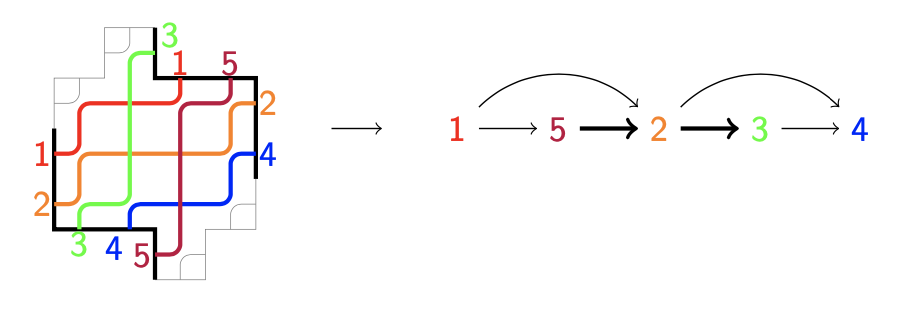
\includegraphics[width=0.52\textwidth]{interval_not_contained1} \quad
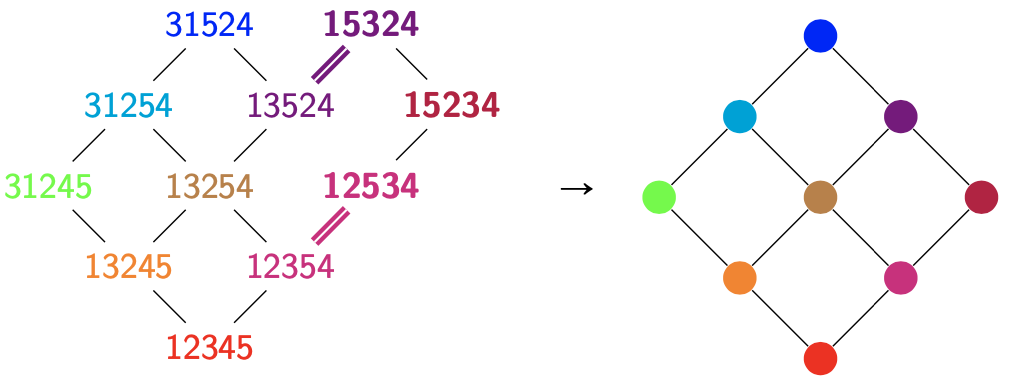
\includegraphics[width=0.43\textwidth]{interval_not_contained2}
\end{figure}
  \setcounter{enumi}{3}
\item $\linearExtensions(I)$ is not an interval in general. See for instance the example~\cite[Figure~9]{PilaudStump-brickPolytope}. 
In that figure, the elements of the week order $\mathfrak{S}_4$ that are linear extensions of the same acyclic facet of a given subword complex are grouped together. Some of the groups in the figure are not intervals.  \\
\end{enumerate}
\end{remark}

We will prove the items of the theorem one by one.

\begin{proof}[Proof of \cref{thm_subword_linearextensions_A} \eqref{thmA_item1}]
Let $\pi\in \linearExtensions(I)$ for some facet $I$.
We need to show that if $\pi'<\pi$ then there exist another facet $I'$ such that $\pi'\in \linearExtensions(I')$.
It is enough to show this when $\pi=\pi' s$ for some $s\in S$ such that $\ell(\pi')<\ell(\pi)$.

By definition, $\pi\in \linearExtensions(I)$ if and only if $\Roots(I)\subseteq \pi(\Phi^+)$.
Now, 
\[
\pi(\Phi^+)= -\Inv(\pi)\sqcup \Ninv(\pi)
\]  
and 
\begin{align*}
    \Inv(\pi') &=\Inv(\pi)\smallsetminus \{\beta\} \\
    \Ninv(\pi') &= \Ninv(\pi) \cup \{\beta\}
\end{align*}
for $\beta=\pi'(\alpha_s)$.
Therefore,
\begin{align*}
    \pi'(\Phi^+) = \pi(\Phi^+) \smallsetminus \{-\beta\} \cup \{\beta\}.
\end{align*}

\begin{center}
\begin{tikzpicture}
\coordinate (a) at (0,0);
\coordinate (b) at (0:2);
\coordinate (c) at (60:2);
\coordinate (d) at (120:2);
\coordinate (e) at (180:2);
\draw (b) node[right] {$\beta$};
\draw (e) node[left] {$-\beta$};
%
\path[fill=green!20] (0,0) --  (60:2) arc(60:180:2) -- cycle;
%
\draw[-stealth,dashed] (a) -- (b);
\draw[-stealth] (a) -- (c);
% \draw[-stealth] (a) -- (d);
\draw[-stealth] (a) -- (e);
\node at (120:1) {$\pi(\Phi^+)$};
\end{tikzpicture} 
%
\qquad
%
\begin{tikzpicture}
\coordinate (a) at (0,0);
\coordinate (b) at (0:2);
\coordinate (c) at (60:2);
\coordinate (d) at (120:2);
\coordinate (e) at (180:2);
\draw (b) node[right] {$\beta$};
\draw (e) node[left] {$-\beta$};
%
\path[fill=green!20] (0,0) -- (0:2) arc(0:120:2)  -- cycle;
%
\draw[-stealth] (a) -- (b);
% \draw[-stealth] (a) -- (c);
\draw[-stealth] (a) -- (d);
\draw[-stealth,dashed] (a) -- (e);
\node at (60:1) {$\pi'(\Phi^+)$};
\end{tikzpicture} 
\end{center}
%
Note that the reflection $s_\beta=\pi's\pi'^{-1}$ orthogonal to the root $\beta$ transforms $\pi(\Phi^+)$ and $\pi'(\Phi^+)$ into each other:
\[
s_\beta(\pi(\Phi^+))=\pi'(\Phi^+).
\]
Since $s_\beta(\beta)= -\beta$, then $s_\beta$ preserves the set 
\[
\pi(\Phi^+)\smallsetminus \{-\beta\}=
\pi'(\Phi^+)\smallsetminus \{\beta\}=
\pi(\Phi^+)\cap \pi'(\Phi^+).
\]
This observation will be useful to prove the statement in the second of the following two cases.

\medskip
{\bf Case 1}: $-\beta \notin \Roots(I)$.

In this case, 
$\Roots(I)\subseteq \pi(\Phi^+) \smallsetminus \{-\beta\} \subseteq \pi'(\Phi^+)$.
Taking $I'=I$, we have 
$\pi'\in \linearExtensions(I')$ 
as wanted.

\medskip
{\bf Case 2}: $-\beta \in \Roots(I)$.

In this case, we need to remove $-\beta$ from the root configuration.
We will achieve this by flipping the position of the last $-\beta$ in $I$ to create a new facet $I'$.
This position is indeed flippable as we will argue now. 

Given a facet $I$ of a subword complex~$\subwordComplex(Q,w)$ and a positive root $\beta\in \Phi^+$, the restriction of the list of roots 
\[
\rootFunction{I}{1}, \rootFunction{I}{2}, \dots , \rootFunction{I}{m}.
\]
to the set $\{\beta,-\beta\}$ is of the form
\[
\begin{array}{cccc}
  \beta, \dots , & \beta &, -\beta, \dots, &-\beta.\\
     & i && j
\end{array}
\]
The sequence of $-\beta$'s could in principle be empty and so does the sequence of $\beta$'s.
But if there is a $-\beta$ in this list, then there should be at least one $\beta$ preceding it.
The position $i$ of the last $\beta$ is used in the reduced expression of $w$ in the complement of $I$, that is $i\notin I$.
The positions of the other $\beta$'s and $-\beta$'s all belong to~$I$, and can all be flipped to $i$ (see \cref{lem_rootfunction_flips}~\eqref{lem_rootfunction_flips2}).   
In particular, the position $j$ of the last $-\beta$ belongs to $I$, and it can be flipped to $i$ creating a new facet $I'=I\smallsetminus \{j\} \cap \{i\}$.

Now, since $\beta\notin \pi(\Phi^+)$.
There must be only one $\beta$ in the list.
Otherwise, there would be at least one $\beta$ whose position belongs to the facet $I$.
This would imply that $\beta\in \Roots(I)$ and $\pi$ would not be a linear extension of $I$, which is a contradiction.
So, our restricted list corresponding to $I$ looks like
\begin{equation}
\begin{array}{ccc}
  \beta &, -\beta, \dots, &-\beta.\\
      i && j
\end{array}    
\end{equation}
Flipping $j$ to $i$ creates the new facet $I'=I\smallsetminus \{j\} \cap \{i\}$ whose corresponding restricted list looks like
\begin{equation}
\begin{array}{ccc}
  \beta &, \beta, \dots, &\beta.\\
      i && j
\end{array}    
\end{equation}
Indeed, Equation~\eqref{eq_rootfunction_flip} describes how the root function is modified after a flip.
For a position $k$ satisfying $i<k\leq j$, we have $\rootFunction{I'}{k}=s_\beta (\rootFunction{I}{k})$; otherwise we have $\rootFunction{I'}{k}=\rootFunction{I}{k}$.
Then, all $-\beta$'s get transformed into $\beta$'s.

Moreover, since the reflection $s_\beta$ preserves the set 
$$\pi'(\Phi^+)\smallsetminus \{\beta\} =
\pi(\Phi^+)\smallsetminus \{-\beta\} =
\pi(\Phi^+) \cap \pi'(\Phi^+).
$$
then $\Roots(I')\subseteq \pi'(\Phi^+)$.
Thus, $\pi'\in \linearExtensions(I')$ as desired.
\end{proof}

\begin{proof}[Proof of \cref{thm_subword_linearextensions_A}~\eqref{thmA_item2}]
By part \eqref{thmA_item1}, the union of all linear extensions of facets is a lower set.
So, we just need to show that $w$ belongs to this set.
This follows from $w\in \linearExtensions(\antiGreedyFacet)$, which was proven in \cref{lem_linearext_greedyfacets}.
\end{proof}

\begin{proof}[Proof of \cref{thm_subword_linearextensions_A}~\eqref{thmA_item3}]
We will show that if there is an element $\pi\in \linearExtensions(I_1)\cap \linearExtensions(I_2)$ then $I_1= I_2$.
We already showed this for $\pi=e$ in \cref{lem_linearext_greedyfacets}.

Let $I_1, I_2$ be two facets such that $e\neq \pi \in \linearExtensions(I_1)\cap \linearExtensions(I_2)$.
As in the proof of part \eqref{thmA_item1}, let $\pi'=\pi s$ for some $s\in S$ such that $\ell(\pi')<\ell(\pi)$, and let $I_1',I_2'$ be the corresponding facets obtained using the same steps of the proof.
These new facets satisfy $\pi'\in \linearExtensions(I_1')\cap \linearExtensions(I_2')$.

We claim that $I_1=I_2$ if and only if $I_1'=I_2'$.
The forward direction is clear.
For the reverse direction we analyze the two cases if the proof of part \eqref{thmA_item1}.
Note that in Case~1, the resulting facet~$I'$ obtained from $I$ satisfies $\beta\notin \Roots(I')$, while in Case 2 we have $\beta \in \Roots(I')$. 
Therefore, if $I_1'=I_2'$ then both $I_1$ and $I_2$ fall into Case 1 or both into Case 2.
If both fall into Case 1, then $I_1'=I_1$ and $I_2'=I_2$ and so $I_1=I_2$ as desired.
If both fall into Case 2, then we just need to flip back the performed flip to obtain $I_1=I_2$.

Now we need to show that $I_1=I_2$.
We proceed by contradiction.
If $I_1\neq I_2$, then $I_1'\neq I_2'$ and $\pi'\in \linearExtensions(I_1')\cap \linearExtensions(I_2')$.
We can continue going down in the week order until reaching the minimal element $e$.
The resulting two facets are different and their linear extensions contain $e$.
This is a contradiction to \cref{lem_linearext_greedyfacets}.  
\vincent{This paragraph is not needed. Say it better in the first paragraph of the proof of (3).}
\end{proof}

\begin{proof}[Proof of \cref{thm_subword_linearextensions_A}~\eqref{thmA_item4}]
Let $\pi_1,\pi_2\in \linearExtensions(I)$ and assume $\pi_1<\pi_2$.
We need to show that if $\pi_1\leq \pi \leq \pi_2$ then~$\pi \in \linearExtensions(I)$.
By definition of linear extensions and \cref{lem_pi_phiplus_inv_ninv} we have
\[
\Roots(I) \subseteq \pi_i(\Phi^+)=-\Inv(\pi_i)\sqcup \Ninv(\pi_i)
\]
for $i=1,2$.
Restricting to the set of negative and positive roots, respectively, we deduce
\[
\Roots(I)\cap \Phi^- \subseteq -\Inv(\pi_1) \subseteq -\Inv(\pi) \qquad 
\Roots(I)\cap \Phi^+ \subseteq \Ninv(\pi_2)  \subseteq \Ninv(\pi)
\]
Therefore
\[
\Roots(I) \subseteq \pi(\Phi^+)=-\Inv(\pi)\sqcup \Ninv(\pi)
\]
and so $\pi\in \linearExtensions(I)$.
\end{proof}



For simplicity, we denote by 
\[
\linearExtensions(Q,w) = \bigcup_{I\in\subwordFacets(Q,w)} \linearExtensions(I)
\]
the \defn{set of linear extensions of all facets} of $\subwordComplex(Q,w)$.
Since $\linearExtensions(I)\neq \varnothing$ if and only if $I$ is acyclic (\cref{lem_acyclic_nonempty}), we have the following straight forward corollary.

\begin{corollary}\label{cor_linearextensions_partition}
The following holds:    
\begin{align}
    \linearExtensions(Q,w) =
    \bigsqcup_{I\in\subwordAcyclicFacets(Q,w)} \linearExtensions(I).
\end{align}
\end{corollary}

As pointed out in \cref{rem_thmA}, there are subword complexes for which $[e,w] \neq \bigcup_{I\in\subwordFacets(Q,w)}$.
Our second fundamental theorem describes a large family of cases where equality holds.

\begin{theorem}\label{thm_subword_linearextensions_B}

Let $\subwordComplex(Q,w)$ be a non-empty subword complex such that the word $Q$ contains a reduced expression of $\wo$.
The linear extensions of acyclic facets of $\subwordComplex(Q,w)$ form a partition of the interval $[e,w]$:
\begin{align}
    [e,w] =
    \bigsqcup_{I\in\subwordAcyclicFacets(Q,w)} \linearExtensions(I).
\end{align}
\end{theorem}

The proof of this theorem is based on the following proposition, which follows from~\cite[Theorem~3.1 and Corollary 3.3]{JahnStump}.

\begin{proposition}[{\cite{JahnStump}}]\label{prop_jahnStump_intersection}
    Let $\subwordComplex(Q,w)$ be a non-empty subword complex such that the word $Q$ contains a reduced expression of $\wo$.
Then 
    \[
\left(
\bigcap_{I\in \subwordFacets(Q,\pi)} \cone \Roots(I) 
\right)
\cap \Phi
= 
\Ninv(w).
    \]
\end{proposition}
\begin{proof}
    We include a short proof here for self containment.
We refer to~\cite{JahnStump} for the description of the notation $C^+(w,\cdot)$.
    By~\cite[Theorem~3.1]{JahnStump} we have
    \[
\bigcap_{I\in \subwordFacets(Q,\pi)} \cone \Roots(I) =
C^+(w,\DemazureProduct(Q)).
    \]
    The word $Q$ contains a reduced expression of $\wo$ if and only if $\DemazureProduct(Q)=\wo$.
Furthermore, by~\cite[Corollary~3.3]{JahnStump} we have
    \[
C^+(w,\wo)\cap \Phi
= \Inv(w \wo) = \Ninv(w).
    \]    
\end{proof}

\begin{proof}[Proof of \cref{thm_subword_linearextensions_B}]
Assume $\pi\in \linearExtensions(I)$.
We want to show that $\pi<w$.
By \cref{prop_jahnStump_intersection} we have 
\[
\Ninv(w) 
\subseteq \cone \Roots(I) 
\subseteq \cone \pi(\Phi^+).
\]
Therefore
\[
\Ninv(w) 
\subseteq \cone \pi(\Phi^+) \cap \Phi^+ 
= \Ninv(\pi).
\]
Thus $\pi \leq w$ as desired.
\end{proof}




\subsection{The sweeping algorithm}

Given a linear extension $\pi \in \linearExtensions(Q,w)$, one natural question is whether we can recover the unique acyclic facet $I$ such that $\pi \in \linearExtensions(I)$.
We can recover this facet via a sweeping algorithm which we now introduce.
The algorithm outcomes a facet for every element~$\pi \in W$, and this will be the desired facet for each $\pi \in \linearExtensions(Q,w)$.

\[
\begin{tabular}{cccc}
$\sweepingAlgorithm$ : & $W$  &$\longrightarrow$ &$\subwordFacets(Q,w)$\\
    & $\pi$ & $\longrightarrow$ & $\sweepingAlgorithm(Q,w,\pi)$
\end{tabular}
\]



We start by setting $I^0=\varnothing$ to be the empty set.
Then we scan the word $Q=(q_1,\dots ,q_m)$ from left to right.
At position $j\in [m]$ we produce a new set $I^j$ obtained from the previous one $I^{j-1}$ by either adding $j$ or not, according to certain rules.
We let $Q^j=Q_{[j]\smallsetminus I^j}$ and denote by
    \[
    \rootFunction{I^j}{k} = \prod Q_{[k-1]\smallsetminus I^j}(\alpha_{q_k}).
    \]
the partial root function for $k\leq j$.  
The rules are the following:

\begin{enumerate}
    \item If $\rootFunction{I^j}{j}\in \Ninv(w)$ then let 
    \[
    I^j=I^{j-1}\cup\{j\}.
    \] 
    \label{sweeping_case1}
    \item If $\rootFunction{I^j}{j}\in \Inv(w) \cap \Inv (\pi)$ then let 
    \[
    I^j=I^{j-1}.
    \]
    \label{sweeping_case2}
    \item If $\rootFunction{I^j}{j}\in \Inv(w) \cap \Ninv (\pi)$ then we consider two cases: 
    \label{sweeping_case3} 
    \begin{enumerate}
        \item If $Q_{[m]\smallsetminus I^{j-1}\smallsetminus \{j\}}$ contains a reduced expression of $w$ with prefix $Q^{j-1}$ then let 
        \[
        I^j=I^{j-1}\cup \{j\}.
        \]        
        \label{sweeping_case3a}
        \item If not let 
        \[
        I^j=I^{j-1}.
        \]
        \label{sweeping_case3b}
    \end{enumerate}
    \item If $\rootFunction{I^j}{j}\in -\Inv(w)$ then let
    \[
    I^j=I^{j-1}\cup \{j\}.
    \]
    \label{sweeping_case4}
\end{enumerate}

We denote by \defn{$\sweepingAlgorithm(Q,w,\pi)$} the resulting set $I^m$ obtained at the last step of the algorithm.

Roughly speaking, the goal of the algorithm is to insert a reduced expression of $w$ in $Q$ by sweeping the word from left to right, while deciding whether we use a letter or not by looking at the root $\beta=\rootFunction{I^j}{j}$ that it produces.
If $\beta \in \Ninv(w)$ then it can not be used (Case~\eqref{sweeping_case1}), otherwise we would not have a reduced expression for $w$.
If $\beta \in \Inv(w)$ then we take it when $\beta \in \Inv(\pi)$ (Case~\eqref{sweeping_case2}), or delay it as much as possible when $\beta \in \Ninv(\pi)$ (Case~\eqref{sweeping_case3}).
If $\beta \in -\Inv(w)$ we can simply not take it (Case~\eqref{sweeping_case4}).

\begin{proposition}
\label{prop_sweeping1}
    Let $\subwordComplex(Q,w)$ be a non-empty subword complex.
    For every $\pi \in W$, the set $\sweepingAlgorithm(Q,w,\pi)$ is a facet of $\subwordComplex(Q,w)$.
\end{proposition}

\begin{proof}
    Let $I^j$ and $Q^j=Q_{[j]\smallsetminus I^j}$ be as defined in the sweeping algorithm for $\pi$. 
    The proposition follows by applying the following claim for $j=m$.
    \smallskip
    
    {\bf Claim}: $Q^j$ is a reduced expression which is the prefix of a reduced expression of $w$ in $Q_{[m]\smallsetminus I^j}$.

    \smallskip
    We prove the claim by induction on $j$.

    For $j=0$, $Q^0$ is the empty word which is reduced by definition.
    Furthermore, $Q_{[m]\smallsetminus I^0 }=Q$ contains a reduced expression of $w$ because the subword complex is non-empty.
The empty word is a prefix of this reduced expression. 

    Now assume that the claim holds for $j-1$ and prove it for $j$.
    Note that 
    \begin{equation}
         Q^j = 
  \begin{cases}
    Q^{j-1}, & \text{if } I^j=I^{j-1}\cup \{j\} \\
    Q^{j-1}\circ (q_j), & \text{if } I^j=I^{j-1}
  \end{cases}
    \end{equation}    
    We analyze the different cases of the sweeping algorithm.
    \begin{enumerate}
    \item If $\rootFunction{I^j}{j}\in \Ninv(w)$ then 
    $Q^j=Q^{j-1}$, which is reduced by induction hypothesis.
    Moreover, it is a prefix of a reduced expression of $w$ in $Q_{[m]\smallsetminus I^{j-1}}$.
    Since $\rootFunction{I^j}{j}\in \Ninv(w)$, this reduced expression can not use the letter $q_j$; so, it is a reduced expression of $w$ in $Q_{[m]\smallsetminus I^{j}}$ as desired.
    \item If $\rootFunction{I^j}{j}\in \Inv(w) \cap \Inv (\pi)$ then $Q^j= Q^{j-1}\circ (q_j)$, which is a reduced expression because~$Q^{j-1}$ is reduced and $\rootFunction{I^j}{j}\in \Inv(w)$.
    
    Now let $\widetilde Q$ be a subword of $Q_{[m]\smallsetminus I^{j-1}}=Q_{[m]\smallsetminus I^{j}}$ which is a reduced expression of $w$ with prefix $Q^{j-1}$, and let $\widetilde I$ be the corresponding facet.
    
    If $j\notin \widetilde I$, then $q_j$ is used in $\widetilde Q$ and we are done because $\widetilde Q$ has $Q^j$ as a prefix.

    If $j\in \widetilde I$, then we can flip it to a position $j'>j$ (by \cref{lem_rootfunction_flips}~\eqref{lem_rootfunction_flips2}), creating a new reduced expression $\widetilde Q'$ of $w$ which uses $q_j$, and thus has $Q^j$ as a prefix.


    \item[(3)(a)] If $\rootFunction{I^j}{j}\in \Inv(w) \cap \Ninv (\pi)$ and $Q_{[m]\smallsetminus I^{j-1}\smallsetminus \{j\}}$ contains a reduced expression of $w$ with prefix $Q^{j-1}$, then $Q^j=Q^{j-1}$.
    Therefore, $Q^j$ is reduced and it is a prefix of a reduced expression of $w$ in 
    $Q_{[m]\smallsetminus I^{j-1}\smallsetminus \{j\}}=Q_{[m]\smallsetminus I^j}$.

    \item[(3)(b)] In this case, $\rootFunction{I^j}{j}\in \Inv(w) \cap \Ninv (\pi)$ but $Q^j= Q^{j-1}\circ (q_j)$. The proof is similar to the proof of (2).

    \item[(4)] If $\rootFunction{I^j}{j}\in -\Inv(w)$ then $Q^j=Q^{j-1}$. The argument is similar to that of part (1).
    \end{enumerate}

Finally, we need to argue that any position $j$ falls into one of these cases.
The root $\rootFunction{I^j}{j}\in \Phi^+ \sqcup \Phi^-$ and we know that
\[
\Phi^+ = \Inv(w) \sqcup \Ninv(w) \qquad \qquad
\Phi^- = -\Inv(w) \sqcup -\Ninv(w)  
\]
The positive roots are covered by the cases (1),(2), and (3).
The negative roots in $-\Inv(w)$ are covered in case (4).
Since we are inserting a reduced expression of $w$ in $Q$, the case $-\Ninv(w)$ never occurs. 
\end{proof}

The following proposition shows that for every linear extension $\pi \in \linearExtensions(Q,w)$, the sweeping algorithm recovers the unique acyclic facet $I$ such that $\pi \in \linearExtensions(I)$.

\begin{proposition}
\label{prop_sweeping2}
    If $\pi\in \linearExtensions(I)$ for some facet $I\in \subwordComplex(Q,w)$, then 
    \[
I = \sweepingAlgorithm(Q,w,\pi).
    \]
\end{proposition}

Our proof is based on the following lemma.

\begin{lemma}\label{lem_negativeroot}
    Let $I_1,I_2\in \subwordComplex(Q,w)$ be two different facets, and $j\in [m]$ be the first position where they differ.
    Without loss of generality assume 
    \[
I_2\cap [j] = I_1\cap [j] \smallsetminus \{j\}
    \]
with $j\in I_1$.
Let $\beta=\rootFunction{I_1}{j}=\rootFunction{I_2}{j}$, then 
\[
-\beta \in \cone \Roots(I_2).
\]
\end{lemma}

\begin{proof}
    ~\cesar{Noemie: can you please write the proof of this Lemma? I do not remember the details at the moment, but the proof is based on the paper of Jahn--Stump that we discussed during your visit in Graz.}
\end{proof}

\begin{proof}[Proof of \cref{prop_sweeping2}]
Assume $\pi \in \linearExtensions(I)$ and let $I^j=I\cap [j]$.
We will show that the partial root function $\rootFunction{I^j}{\cdot}$ agrees with the decisions taken in the sweeping algorithm.
Indeed, we will see that those decisions are forced.

Recall that 

\begin{center}
\begin{tabular}{ccl}
    $\pi \in \linearExtensions(I)$ & $\longleftrightarrow$ & $R(I)\subseteq \pi(\Phi^+)$\\
     & $\longleftrightarrow$ & $\cone R(I)\subseteq \pi(\Phi^+)$
\end{tabular}    
\end{center}
and 
\[
\pi(\Phi^+) = -\Inv(\pi) \sqcup \Ninv(\pi).
\]
We analyze the possible cases in the sweeping algorithm.

\begin{enumerate}
    \item If $\rootFunction{I^j}{j}\in \Ninv(w)$ then clearly $j\in I$ is forced. Otherwise $Q_{[m]\smallsetminus I}$ would not be a reduced expression of $w$.
    \item If $\rootFunction{I^j}{j}\in \Inv(w) \cap \Inv (\pi)$ then $j\notin I$ is forced. 
    Otherwise we would have an inversion of $\pi$ in the root configuration, which contradicts $\pi \in \linearExtensions(I)$.
    \item[(3)(a)] If $\rootFunction{I^j}{j}\in \Inv(w) \cap \Ninv (\pi)$ and $Q_{[m]\smallsetminus I^{j-1}\smallsetminus \{j\}}$ contains a reduced expression of $w$ with prefix $Q^{j-1}$ then $j\in I^j$ is forced. 

    We argue this by contradiction. 
    Assume $j\notin I^j$ ($j\notin I$). Let $I_1=\sweepingAlgorithm(Q,w,\pi)$ and $I_2=I$. Applying \cref{lem_negativeroot}, we deduce that $\beta=\rootFunction{I^j}{j}=\rootFunction{I}{j}$ satisfies 
    \[
    -\beta \in \cone \Roots(I).
    \]
    But $\beta \in \Ninv(\pi)$. This contradicts $\pi\in \linearExtensions(I)$.
    \item[(3)(b)]  If $\rootFunction{I^j}{j}\in \Inv(w) \cap \Ninv (\pi)$ and $Q_{[m]\smallsetminus I^{j-1}\smallsetminus \{j\}}$ does not contain a reduced expression of $w$ with prefix $Q^{j-1}$ then $j\notin I^j$ is forced. Otherwise, the complement of $I$ would not be a reduced expression of $w$.
    \item[(4)] If $\rootFunction{I^j}{j}\in -\Inv(w)$ then $j\in I^j$ is clearly forced. Otherwise, the complement of $I$ would not be a reduced expression.
\end{enumerate}
\end{proof}

\begin{remark}
    Although the sweeping algorithm produces a facet $I=\sweepingAlgorithm(Q,w,\pi)$ for every~$w\in W$, in some cases we have $\pi \notin \linearExtensions(I)$. 
    This happens because of Case~\eqref{sweeping_case1}, when a non-inversion~$\beta\in \Ninv(w)$ of $w$ is added to the root configuration $\Roots(I)$, such that~$\beta \notin \Ninv(\pi)$. This is only potentially possible when $\pi \notin [e,w]$.
\end{remark}


\subsection{The subword complex congruence conjecture}\cesarm{To do: meet to discuss about this section? put it in final form...}
By \cref{cor_linearextensions_partition}, the set $\linearExtensions(Q,w)$ of linear extensions of all facets of $\subwordComplex(Q,w)$ can be written as
\begin{align*}
    \linearExtensions(Q,w) =
    \bigsqcup_{I\in\subwordAcyclicFacets(Q,w)} \linearExtensions(I).
\end{align*}
This partition determines a natural equivalence relation on the set $\linearExtensions(Q,w)$.

\begin{definition}
For a non-empty subword complex $\subwordComplex(Q,w)$, the \defn{subword complex congruence} is the equivalence relation~$\equiv_{Q,w}$ on the set $\linearExtensions(Q,w)\subseteq W$ of linear extensions  of all facets of $\subwordComplex(Q,w)$ determined by $\pi \equiv_{Q,w} \pi'$ if and only if $\pi$ and $\pi'$ are linear extensions of the same facet.  
\end{definition}

By \cref{thm_subword_linearextensions_B}, if $Q$ contains a reduced expression for $\wo$, this gives an equivalence relation on the interval $[e,w]$ of the week order.
We say that a word $Q$ is \defn{alternating} if all non-commuting pairs $s, t\in S$ alternate within $Q$.
The following conjecture is supported by extensive computer computations.\cesarm{Noemie: in which cases did you check this conjecture? Type $A_n$ for n=???, B,C,D,....?} 

\begin{conjecture}
Let $Q$ be an alternating word which contains a reduced expression for $\wo$.
For any~$w\in W$, the subword complex congruence~$\equiv_{Q,w}$ is a lattice congruence of the interval~$[e,w]$ of the weak order.
\end{conjecture}
\cesarm{Do we have more conjectures or questions to be included here?}








\begin{remark}\label{rem_acyclicflipposet_not_latticequotient}
In analogy to the case of pipe dreams in \cref{subsec:proofCongruence}, one might expect that the quotient~$[e,\omega]/\equiv_{Q,w}$ is isomorphic to the restriction of the increasing flip poset of $\subwordComplex(Q,w)$ to the set of acyclic facets.
But this is not the case as shown in \cref{ex_acyclicflip_not_weakorder_related}.     
\end{remark}

\begin{example}\label{ex_acyclicflip_not_weakorder_related}
    Let $W=S_3$ be the symmetric group generated by simple transpositions $S=\{s_1,s_2\}$ with $s_i=(i, i+1 )$.
Let $Q=(s_1,s_2,s_1,s_2,s_1,s_2)$ and $w=\wo=s_1s_2s_1=s_2s_1s_2$.
The subword complex $\subwordComplex(Q,w)$ has eight facets, six of which are acyclic.
    All the fibers of $\equiv_{Q,w}$ are singletons and the lattice quotient~$[e,\omega]/\equiv_{Q,w}$ coincides with the weak order of type $A_2$.
    On the other hand there are two facets, $I_1=\{1,3,4\}$ and $I_2=\{3,4,6\}$, which are connected by a flip but whose corresponding elements $\pi_1$ and $\pi_2$ are not related in weak order.
    \cesar{To do: Double check and expand this example in detail. Add figure.}
\end{example}

As we have seen in \cref{cor_acyclicpipedreams_lattice}, the increasing flip poset of acyclic pipe dreams of any permutation $w$ is a lattice, because it is isomorphic to the lattice quotient~$[e,\omega]/\equiv_\omega$.
This motivates the following open question for subword complexes.

\begin{question}
Let $\subwordComplex(Q,w)$ be a non-empty subword complex.
Is the restriction of the increasing flip poset of $\subwordComplex(Q,w)$ to the set of acyclic facets a lattice?    
\end{question}

As pointed out in \cref{rem_acyclicflipposet_not_latticequotient},  we can not expect~$[e,\omega]/\equiv_{Q,w}$ to be isomorphic to the restriction of the increasing flip poset of $\subwordComplex(Q,w)$ to the set of acyclic facets.
\cref{ex_acyclicflip_not_weakorder_related} shows that there are flips between acyclic facets that are not detected by the week order.
One could expect that there is a natural restriction to a special class of flips that behave nicer, meaning that all of them are identified by the quotient~$[e,\omega]/\equiv_{Q,w}$.
In our \cref{ex_acyclicflip_not_weakorder_related}, the generalized Chute moves from~\cite{Rubey} do the job, because the flip that is not detected by the week order is exactly the one flip which is not Chute.
The Chute lattice conjecture~\cite[Conjecture~2.8]{Rubey} might be an indication that this is the right direction to look at.



%%%%%%%%%%%%%%%%%%%%%%%%%%%%%%%%%%%%%%
%%%%%%%%%%%%%%%%%%%%%%%%%%%%%%%%%%%%%%
%%%%%%%%%%%%%%%%%%%%%%%%%%%%%%%%%%%%%%

\bibliographystyle{alpha}
\bibliography{latticePipeDreams}
\label{sec:biblio}

%%%%%%%%%%%%%%%%%%%%%%%%%%%%%%%%%%%%%%

\end{document}
